%======================================================================
%  Nonlinear Methods in Mechanics -- exercise session, Chapter 3
%  A. Constantinescu, LMS, CNRS & Ecole Polytechnique
%
%  One PDF, in the order of use:
%    1. the session sheet (questions only, at most 8 pages: printed)
%    2. the guides of the three codes, same blocks and same structure:
%       Cast3M, FEniCS, Python
%    3. the session sheet with the answers (at the end, to cut out)
%  The sheet is written once (ch3/sheet.tex) and printed twice: the
%  answer environments are shown only in the second copy.
%
%  Build: compile the book first (its .aux files give the numbers cited
%  here), then in this directory `latexmk -pdf session_ch3'
%  (.latexmkrc puts the repository root on TEXINPUTS).
%======================================================================
\documentclass[11pt,a4paper,oneside,openany]{book}

\usepackage{xr-hyper}          % before hyperref (loaded by the style)
\input{preamble/style}
\input{preamble/notation}
%======================================================================
%  session_preamble.tex -- what the exercise sessions add to the shared
%  preamble of the notes (preamble/style.tex, notation.tex)
%======================================================================

\usepackage{environ}

%---- page header: course, year, chapter ---------------------------------
\newcommand{\sessioncourse}{Nonlinear Methods in Mechanics -- 2026}
\newcommand{\sessionchapter}{}            % set by each session
\fancypagestyle{session}{%
  \fancyhf{}%
  \fancyhead[L]{\sffamily\small\sessioncourse}%
  \fancyhead[R]{\sffamily\small\sessionchapter}%
  \fancyfoot[C]{\sffamily\small\thepage}%
  \renewcommand{\headrulewidth}{0.4pt}}

% title block of a sheet (no title page: the sheet is printed)
\newcommand{\sessiontitle}[2]{%
  \thispagestyle{session}%
  \begin{center}
  {\sffamily\bfseries\Large \sessioncourse\par}\vspace{1.5mm}
  {\sffamily\bfseries\large #1\par}\vspace{1mm}
  {\sffamily Andrei CONSTANTINESCU --
   \texttt{andrei.constantinescu@polytechnique.edu}\par}\vspace{1mm}
  {\sffamily\small #2\par}
  \end{center}
  {\color{gray!55}\hrule height 0.4pt}\medskip}

%---- parts a, b, ... and questions a.1, a.2, ... ------------------------
\newcounter{spart}
\renewcommand{\thespart}{\alph{spart}}
\newcounter{sq}[spart]
\makeatletter
\newcommand{\spart}[1]{\par\addvspace{2.2ex plus .5ex}%
  \refstepcounter{spart}%
  {\noindent\sffamily\bfseries\large\thespart.\quad #1\par}%
  \nobreak\vspace{0.6ex}\nobreak\@afterheading}
\makeatother
\newcommand{\q}{\par\smallskip\noindent\refstepcounter{sq}%
  {\sffamily\bfseries\thespart.\arabic{sq}}\quad}
% a question done with the codes
\newcommand{\qc}{\par\smallskip\noindent\refstepcounter{sq}%
  {\sffamily\bfseries\thespart.\arabic{sq}\,\textcolor{cu}{[code]}}\quad}

%---- answers: printed only in the second copy of the sheet --------------
\newif\ifanswers
\NewEnviron{answer}{\ifanswers\par\smallskip
  \begingroup\small\noindent
  {\sffamily\bfseries\color{cphi!80!black}Answer.}\ \BODY\par
  \endgroup\medskip\fi}

% a gibiane operator or keyword in the running text
\providecommand{\op}[1]{\texttt{#1}}

%---- guides -------------------------------------------------------------
\lstdefinestyle{shstyle}{language=bash,
  basicstyle=\ttfamily\scriptsize,
  backgroundcolor=\color{gray!6},frame=none,
  breaklines=true,showstringspaces=false,
  xleftmargin=0.6em,aboveskip=4pt,belowskip=4pt}
\newcommand{\guidesec}[1]{\par\addvspace{2.5ex plus .5ex}%
  {\noindent\sffamily\bfseries\large #1\par}%
  \nobreak\vspace{0.5ex}\nobreak}
\newcommand{\block}[1]{\par\smallskip\noindent{\sffamily\bfseries #1}\quad}
% a status line (shown in red under \drafttrue)
\newcommand{\untested}[1]{\draftnote{#1}}

\externaldocument[B-]{main}    % labels of the book: \ref{B-sec:rg-gap}

\renewcommand{\sessionchapter}{Chapter 3 -- Reciprocity}
\drafttrue        % \draftfalse hides the red status notes

\begin{document}
\pagestyle{session}

%---- 1. the session sheet, questions only ------------------------------
\answersfalse
%======================================================================
%  Session sheet, Chapter 3 (reciprocity gap). Printed twice by
%  session_ch3.tex: without and with the answers. No \label here.
%======================================================================
\ifanswers
\sessiontitle{Chapter 3 -- Reciprocity: session sheet with answers}
  {Answers. Numbers from the Python and FEniCS codes (same gmsh mesh,
   $30$ divisions, P2); Cast3M meshes differently and agrees to about
   two digits.}
\else
\sessiontitle{Chapter 3 -- Reciprocity: session sheet}
  {Notes: Chapter~\ref{B-ch:rg}, Sections~\ref{B-sec:rg-gap}--\ref{B-sec:rg-num}.
   Codes: \texttt{rg\_session} in Cast3M, FEniCS or Python (guides at the
   end of this document).}
\fi

\paragraph{The setting.} A conducting rectangle $\Omega=(0,\ell)\times(0,h)$,
$\ell=1.5$, $h=2$, with conductivity $1$, contains an insulating crack
$\Gamma$, the segment from $A=(0.5,\,1.2)$ to $B=(0.8,\,1.35)$
(Figure~a). The crack is unknown to the identification; $A$ and $B$ only
build the mesh and measure the errors. Coordinates are centred,
$\vect X=\vx-\vx_0$, $\vx_0=(0.75,\,1)$. Two kinds of experiments are used.
\begin{itemize}[itemsep=1pt,topsep=2pt]
\item \textbf{E1, electrodes.} $u=0$ on the bottom, $u=h$ on the top, zero
flux on the vertical sides. The potential is measured on the vertical
sides, the flux (current) on the electrodes.
\item \textbf{Turning potential.} $u=\vd_\beta\cdot\vect X$ on the whole
boundary, $\vd_\beta=(\cos\beta,\sin\beta)$, $\beta=0^\circ,15^\circ,
\dots,165^\circ$. Only the flux is measured (Figure~b).
\end{itemize}

\begin{center}
\begin{tikzpicture}[scale=1.3,>=Stealth]
  % (a) experiment E1
  \begin{scope}
  \fill[gray!8] (0,0) rectangle (1.5,2);
  \draw[cu,line width=2pt] (0,0) -- (1.5,0);
  \draw[cu,line width=2pt] (0,2) -- (1.5,2);
  \draw[cphi,line width=1.2pt] (0,0) -- (0,2);
  \draw[cphi,line width=1.2pt] (1.5,0) -- (1.5,2);
  \draw[very thick] (0.5,1.2) -- (0.8,1.35);
  \fill (0.5,1.2) circle (0.8pt) node[left,font=\scriptsize] {$A$};
  \fill (0.8,1.35) circle (0.8pt) node[right,font=\scriptsize] {$B$};
  \draw[->] (0.65,1.275) -- ++(-0.13,0.26) node[above,font=\scriptsize] {$\vn$};
  \node[font=\scriptsize,cu] at (0.75,-0.17) {$u=0$, flux measured};
  \node[font=\scriptsize,cu] at (0.75,2.17) {$u=h$, flux measured};
  \node[font=\scriptsize,cphi,rotate=90] at (-0.22,1) {$\partial_\nu u=0$, $u$ measured};
  \node[font=\scriptsize,cphi,rotate=90] at (1.72,1) {$\partial_\nu u=0$, $u$ measured};
  \fill (0.75,1) circle (0.6pt) node[below,font=\scriptsize] {$\vx_0$};
  \node[font=\sffamily\small] at (0.75,-0.5) {(a) experiment E1};
  \end{scope}
  % (b) turning potential
  \begin{scope}[xshift=3.4cm]
  \fill[gray!8] (0,0) rectangle (1.5,2);
  \draw[cu,line width=2pt] (0,0) rectangle (1.5,2);
  \draw[very thick] (0.5,1.2) -- (0.8,1.35);
  \draw[->,thick] (0.75,1) -- ++(40:0.45) node[right,font=\scriptsize] {$\vd_\beta$};
  \draw (0.95,1) arc (0:40:0.2) node[midway,right,font=\scriptsize] {$\beta$};
  \draw[gray] (0.75,1) -- (1.1,1);
  \node[font=\scriptsize,cu,align=center] at (0.75,-0.22)
    {$u=\vd_\beta\cdot\vect X$ imposed,\\ flux measured};
  \node[font=\sffamily\small] at (0.75,-0.62) {(b) turning potential};
  \end{scope}
  % (c) the line and the coordinates
  \begin{scope}[xshift=6.4cm,yshift=0.2cm]
  \draw[gray] (-0.2,0.4) -- (1.9,1.45);
  \draw[very thick] (0.6,0.8) -- (1.2,1.1);
  \draw[->] (0.9,0.95) -- ++(0.36,0.18) node[right,font=\scriptsize] {$\vt$};
  \draw[->] (0.9,0.95) -- ++(-0.18,0.36) node[above,font=\scriptsize] {$\vn$};
  \fill (0,0) circle (0.8pt) node[below,font=\scriptsize] {$\vx_0$};
  \draw[dashed] (0,0) -- (-0.2,0.4) node[midway,left,font=\scriptsize] {$c$};
  \node[font=\scriptsize,align=left,anchor=west] at (-0.3,-0.5)
    {line $\vn\cdot\vect X=c$,\\ $s=\vt\cdot\vect X$,\ $\eta=\vn\cdot\vect X-c$};
  \node[font=\sffamily\small] at (0.75,-1.0) {(c) coordinates};
  \end{scope}
\end{tikzpicture}
\end{center}

\paragraph{The codes.} The three versions have the same ten blocks, and they
print and draw the same quantities: 0 parameters; 1 mesh with two lips;
2 model and centred coordinates (FIG~1); 3 procedures; 4 experiment E1 and
its opening (FIG~2--3); 5 measurement; 6 linear and quadratic adjoint
fields; 7 polynomial fields and dipole (FIG~4--5); 8 Fourier and
sine--sinh fields (FIG~6--7); 9 turning potential and the matrix of the
experiments (FIG~8--9). Questions marked \textcolor{cu}{[code]} use them;
the others are done by hand. Run first with exact data (\texttt{eps = 0}).

%======================================================================
\spart{Direct and inverse problem -- recall of the reciprocity gap}
\begin{gbox}{Recall (Notes, Sections \ref{B-sec:rg-direct}--\ref{B-sec:rg-gap})}
Direct problem: $\Delta u=0$ in $\OG$, $\partial_nu^\pm=0$ on the lips, $u$ or
$\partial_\nu u$ given on each part of $\partial\Omega$; well posed by
Lax--Milgram. Inverse problem: $u$ \emph{and} $\varphi=\partial_\nu u$ known
on $\partial\Omega$, $\Gamma$ unknown; ill-posed. For $v$ harmonic in $\Omega$:
$\displaystyle \RG(v)=\int_{\partial\Omega}(u\,\partial_\nu v-v\varphi)\dd s=\int_\Gamma\jump u\,\partial_nv\dd s$.
\end{gbox}

\q Write the direct problem of experiment E1 (equation in $\OG$, condition on
the lips, condition on each side of $\Omega$). Which boundary values are
imposed, which are measured? Why does the identification need both?
\begin{answer}
$\Delta u=0$ in $\OG=\Omega\setminus\Gamma$; $\partial_nu^\pm=0$ on the lips;
$u=0$ on $y=0$, $u=h$ on $y=h$, $\partial_\nu u=0$ on $x=0$ and $x=\ell$.
The electrodes impose $u$ and measure the current $\partial_\nu u$; the
insulated sides impose $\partial_\nu u=0$ and measure $u$. After the
experiment both $u$ and $\varphi=\partial_\nu u$ are known on the whole
boundary (complete Cauchy data). $\RG(v)$ integrates
$u\,\partial_\nu v-v\,\varphi$ over $\partial\Omega$: it needs both.
\end{answer}

\q State the weak form of the direct problem. Why are the lip conditions
natural? Which hypothesis of the Lax--Milgram lemma uses the electrodes?
\begin{answer}
Find $u\in H^1(\OG)$, $u=0$ at the bottom and $u=h$ at the top, such that
$\displaystyle \int_{\OG}\nabla u\cdot\nabla v\dd\vx=0$ for every $v\in V=\{v\in
H^1(\OG):\ v=0$ on the electrodes$\}$. Integrating by parts, the boundary
terms are $\displaystyle \int\partial_\nu u\,v$ on the sides and on both lips:
they vanish for every $v$ only if $\partial_\nu u=0$ there. Hence the zero
flux is natural, as on the insulated sides. Coercivity on $V$ follows from
the Poincar\'e--Friedrichs inequality, which needs $u$ imposed on a part
of the boundary of positive length (the electrodes), Notes
Section~\ref{B-sec:rg-direct}.
\end{answer}

\q Let $v$ be harmonic in the uncracked $\Omega$. Apply Green's second
identity in $\OG$ and show
$\displaystyle \RG(v)=\int_{\partial\Omega}(u\,\partial_\nu v-v\,\varphi)\dd s
=\int_\Gamma\jump u\,\partial_nv\dd s$, $\jump u=u^+-u^-$, $+$ on the side
of $\vn$. Watch the normals of $\OG$ on the two lips.
\begin{answer}
$\displaystyle \int_{\OG}(v\Delta u-u\Delta v)=\int_{\partial\OG}(v\,\partial_{\nu'}u
-u\,\partial_{\nu'}v)$ and the left-hand side is $0$. On $\partial\Omega$,
$\nu'=\vnu$. On $\Gamma^+$, $\nu'=-\vn$; on $\Gamma^-$, $\nu'=+\vn$. On the
lips $\partial_{\nu'}u=0$, and $v$, $\partial_nv$ are continuous across
$\Gamma$. The lips give $\displaystyle \int_\Gamma(u^+-u^-)\partial_nv$, hence
$\displaystyle 0=\int_{\partial\Omega}(v\varphi-u\,\partial_\nu v)+\int_\Gamma\jump
u\,\partial_nv$: this is the identity (Notes, eq.~\eqref{B-eq:rg-identity}).
\end{answer}

\q Show that $\RG(1)=0$, that $\RG$ does not change if $u\to u+C$, and that
$\RG(v)=0$ for every $v$ if there is no crack.
\begin{answer}
$\displaystyle \RG(1)=-\int_{\partial\Omega}\varphi=0$, the flux balance of
$\Delta u=0$ in $\OG$ (no flux through the lips).
$\displaystyle C\int_{\partial\Omega}\partial_\nu v=C\int_\Omega\Delta v=0$.
Without crack, $u$ and $v$ are harmonic in $\Omega$ and Green's identity
gives $0$: Maxwell--Betti reciprocity. The gap measures the crack.
\end{answer}

\q \emph{Discrete gap.} The codes compute
$\RG_h(v)=\sum_{i\in\partial\Omega}\bigl(u_i(\mat Kv)_i-q_iv_i\bigr)$, with
$\mat K$ the conductivity matrix of the cracked mesh and $q=\mat Ku$ the
nodal fluxes (reactions). Show that $\RG_h(v)=-\sum_{i\notin\partial\Omega}
u_i(\mat Kv)_i$. Explain why, for a harmonic polynomial $v$ of degree $\le2$
and quadratic elements, only the nodes of the lips contribute, and
$\RG_h(v)=\int_\Gamma\jump{u_h}\,\partial_nv$ exactly.
\begin{answer}
$\mat K$ is symmetric:
$\sum_{\rm all}u_i(\mat Kv)_i=\sum_{\rm all}v_i(\mat Ku)_i=\sum_{i\in
\partial\Omega}q_iv_i$, because $(\mat Ku)_i=0$ at every node where $u$ is not
imposed (inside, insulated sides, lips). Subtracting gives the formula.
A quadratic $v$ is represented exactly by P2 elements, and
$(\mat Kv)_i=\int\nabla v\cdot\nabla\phi_i=-\int\Delta v\,\phi_i+$ boundary
terms of the support of $\phi_i$. With $\Delta v=0$ this vanishes at every
interior node whose support does not touch the crack. At a node of the upper
lip the support has the lip as boundary, with outward normal $-\vn$:
$(\mat Kv)_i=-\int_{\Gamma}\partial_nv\,\phi_i$; at the lower lip the sign is
$+$. Summing,
$\RG_h(v)=\int_\Gamma(u_h^+-u_h^-)\partial_nv$, without discretization error
beyond that of $u_h$. For other $v$ (cubic, exponential) $(\mat Kv)_i\ne0$
inside, and $\RG_h$ carries an error.
\end{answer}

\qc Run Blocks 1--5 (FIG~1--3). Check $\RG(1)\approx0$. Compare
$\displaystyle \int_\Gamma\jump{u_1}$, read on the lips, with the infinite-body
value $\pi a^2E_n$ ($a$ half-length, $E_n=\vE\cdot\vn$). Why is it smaller?
\begin{answer}
$\RG(1)\approx10^{-13}$ (round-off). $\displaystyle \int\jump{u_1}=0.0764$
against $\pi a^2E_n=0.0790$, $3\%$ less. Two reasons: the opening
vanishes at the last node before each tip (the $\sqrt r$ behaviour is
poorly represented: the mesh error), and the finite body with electrodes is
not the infinite plane. FIG~3: the shape is a semi-ellipse, slightly
below the infinite-body curve.
\end{answer}

%======================================================================
\spart{Families of adjoint fields in 2D -- the plane (the normal)}
\begin{gbox}{Recall (Notes, Section \ref{B-sec:rg-rec}, Step 1)}
$\RG(\vd\cdot\vect X)=m_0\,\vd\cdot\vn$, $\displaystyle m_0=\int_\Gamma\jump u$:
$(\RG(X),\RG(Y))=m_0\vn$, sign fixed by $m_0>0$. A uniform field parallel to
the crack opens nothing: blind experiment.
\end{gbox}

\q Show that the harmonic polynomials of degree $k\ge1$ in 2D form a space of
dimension 2, spanned by $\operatorname{Re}z^k$, $\operatorname{Im}z^k$,
$z=x+\mathrm iy$. List them up to degree 3.
\begin{answer}
A homogeneous polynomial of degree $k$ has $k+1$ coefficients; its
Laplacian is homogeneous of degree $k-2$ ($k-1$ coefficients). Harmonicity
gives $k-1$ independent conditions: dimension $2$. $\operatorname{Re}z^k$,
$\operatorname{Im}z^k$ are harmonic (real and imaginary parts of a
holomorphic function) and independent. Degree 1: $x,\ y$; degree 2:
$x^2-y^2,\ 2xy$; degree 3: $x^3-3xy^2,\ 3x^2y-y^3$.
\end{answer}

\q For $v=\vd\cdot\vect X$ show $\RG(v)=m_0\,\vd\cdot\vn$, with
$\displaystyle m_0=\int_\Gamma\jump u$. Deduce $\vn$ and $m_0$ from $\RG(X)$
and $\RG(Y)$. Is the sign of $\vn$ determined?
\begin{answer}
$\partial_nv=\vd\cdot\vn$ is constant on $\Gamma$:
$\RG(v)=\vd\cdot\vn\int\jump u$. Hence $(\RG(X),\RG(Y))=m_0\vn$,
$m_0=|(\RG(X),\RG(Y))|$, $\vn=(\RG(X),\RG(Y))/m_0$. Exchanging the lips
changes $\vn$ and $\jump u$ together: the sign is fixed by the
convention $m_0>0$.
\end{answer}

\q One measures $\RG(X)=-0.0343$, $\RG(Y)=0.0686$. Give $m_0$, $\vn$, the
angle of the crack with the $x$ axis, and the tangent $\vt$ with $(\vt,\vn)$
direct.
\begin{answer}
$m_0=\sqrt{0.0343^2+0.0686^2}=0.0767$, $\vn=(-0.447,\,0.894)$. The crack is
normal to $\vn$: $\vt=(n_2,-n_1)=(0.894,\,0.447)$, angle $\arctan(0.5)=
26.6^\circ$. (Codes: $0.07664$, $(-0.4472,0.8944)$: exact.)
\end{answer}

\q \emph{Blind experiment.} For a uniform field $\vE=(\cos\beta,\sin\beta)$,
for which $\beta$ is the crack invisible? Is E1 blind? Is the field
$(1,0)$ blind?
\begin{answer}
$m_0=|\tM|\,\vE\cdot\vn$ vanishes when $\vE\perp\vn$, i.e.\ $\vE$ parallel to
the crack: $\beta=26.6^\circ$ (mod $180^\circ$). E1 ($\vE=(0,1)$,
$E_n=0.894$) and $(1,0)$ ($|E_n|=0.447$) are not blind; E1 gives the
larger signal.
\end{answer}

\qc Run Block 6. Compare $\vn$ with the true normal; repeat with
\texttt{eps = 0.001} and \texttt{0.01}. Why is the normal exact without
noise, on a coarse mesh?
\begin{answer}
Exact data: $\vn=(-0.4472,0.8944)$, angle error $0.0000^\circ$: $X,Y$ are
of degree 1 (a.5). Over 200 draws the mean angle error is $0.24^\circ$ at
$10^{-3}$ and $2.4^\circ$ at $10^{-2}$: proportional to the noise.
\end{answer}

%======================================================================
\spart{Position -- the line of the crack}
\begin{gbox}{Recall (Step 2; 2D form, Section \ref{B-sec:rg-num})}
$v_2=(\vn\cdot\vect X)^2-(\vt\cdot\vect X)^2$, $\partial_nv_2=2c$ on the line,
$c=\RG(v_2)/\bigl(2\RG(\vn\cdot\vect X)\bigr)$.
\end{gbox}

\q Show that $v_2=(\vn\cdot\vect X)^2-(\vt\cdot\vect X)^2$ is harmonic, that
$\partial_nv_2=2c$ on the line $\vn\cdot\vect X=c$, and that
$c=\RG(v_2)/(2\RG(\vn\cdot\vect X))$. Why is it enough to know $\vn$?
\begin{answer}
In the rotated coordinates $(\sigma,\tau)=(\vt\cdot\vect X,\vn\cdot\vect X)$,
$v_2=\tau^2-\sigma^2$, $\Delta v_2=2-2=0$; $\partial_nv_2=2\tau=2c$ on the line.
So $\RG(v_2)=2c\,m_0$ and $\RG(\vn\cdot\vect X)=m_0$. The field needs only
$\vn$ (and $\vt$), known from Step 1. In 3D the field is
$(\vn\cdot\vect X)^2-\tfrac12\bigl((\vt_1\cdot\vect X)^2+(\vt_2\cdot\vect X)^2\bigr)$.
\end{answer}

\q Why do the codes use centred coordinates $\vect X=\vx-\vx_0$? Estimate
the size of $v_2$ on $\partial\Omega$ with and without centring.
\begin{answer}
By the bound $|\RG(v)|\le\|u\|\,\|\partial_\nu v\|+\|\varphi\|\,\|v\|$ (Notes,
Section~\ref{B-sec:rg-gap}, property (iii)) the noise is amplified by the
size of $v$ on $\partial\Omega$. Centred, $|v_2|\le|\vect X|^2\le
0.75^2+1^2=1.56$; from the corner $(0,0)$, $|\vx|^2$ reaches $1.5^2+2^2=6.25$:
four times larger. $c$ is a ratio of two gaps; a smaller $v_2$ gives
a smaller error on it.
\end{answer}

\qc Run Block 6: $c$ with exact data and with noise. Which point of the line
is it? (FIG~4: green line.)
\begin{answer}
$c=0.2907$, the true value ($v_2$ is of degree 2). It is the distance from
$\vx_0$ to the line, positive on the side of $\vn$. Over 200 draws:
$c=0.2905\pm0.0035$ at $10^{-3}$, $0.289\pm0.036$ at $10^{-2}$.
\end{answer}

%======================================================================
\spart{Extension -- Fourier and sine--sinh adjoint fields}
\begin{gbox}{Recall (Step 3, Sections \ref{B-ssec:rg-step3}--\ref{B-ssec:rg-stab})}
$V_\xi=e^{\xi\eta}e^{-\mathrm i\xi s}$: $\RG(V_\xi)=\xi\hat w(\xi)$. On a bounded
interval: $v_k=\sin(\lambda_kg)\sinh(\lambda_k\eta)/\lambda_k$,
$\displaystyle w=\sum_k\frac2L\RG(v_k)\sin\lambda_kg$. Noise $\delta$: only
$\delta e^{\lambda H}\lesssim1$ is usable, resolution $\pi H/\ln(1/\delta)$.
\end{gbox}

\q With $s=\vt\cdot\vect X$ and $\eta=\vn\cdot\vect X-c$, show that
$V_\xi=e^{\xi\eta}e^{-\mathrm i\xi s}$ is harmonic and that
$\RG(V_\xi)=\xi\,\hat w(\xi)$, $\hat w$ the Fourier transform of the
opening $w(s)$. Write the two real fields used by the codes and what they
give.
\begin{answer}
$\Delta V_\xi=(\xi^2-\xi^2)V_\xi=0$; $\partial_\eta V_\xi=\xi e^{-\mathrm i\xi s}$ at
$\eta=0$, so $\RG(V_\xi)=\xi\int w\,e^{-\mathrm i\xi s}$. Real and imaginary
parts: $e^{\xi\eta}\cos\xi s'$ and $e^{\xi\eta}\sin\xi s'$ ($s'=s-s_0$)
give $\xi C(\xi)$ and $\xi S(\xi)$, with $\displaystyle C=\int w\cos\xi s'$,
$\displaystyle S=\int w\sin\xi s'$.
\end{answer}

\q Why does $\hat w$ known for all $\xi$ determine the crack
(Paley--Wiener)? For a semi-elliptic opening $w=A\sqrt{a^2-s'^2}$ show that
$C(\xi)=2m_0\,J_1(\xi a)/(\xi a)$ (use
$\displaystyle \int_{-a}^a\sqrt{a^2-s^2}\cos\xi s\dd s=\pi aJ_1(\xi a)/\xi$). The
first zero of $J_1$ is $3.832$: at which $\xi$ does $C$ vanish here?
\begin{answer}
$w$ has compact support: $\hat w$ is entire, known from any interval of
$\xi$, and its inverse gives $w$, whose support is $\Gamma$.
$C=A\pi aJ_1(\xi a)/\xi$ and $m_0=\pi Aa^2/2$, hence $C=2m_0J_1(\xi a)/(\xi
a)$. With $a=0.168$: $\xi=3.832/0.168=22.8$.
\end{answer}

\q On $\partial\Omega$, $\eta$ varies between $-1.52$ and $0.94$. Estimate the
largest value of $|V_\xi|$ on the boundary for $\xi=2,\ 4,\ 8,\ 22.8$. With a
relative noise $\delta$ on the data, which $\xi$ are usable?
\begin{answer}
$e^{0.94\xi}$: $6.5$, $43$, $1.8\cdot10^3$, $2\cdot10^9$. The data error on
$\RG$ is about $\delta\,e^{0.94\xi}$ (times $m_0$), against a signal
$\xi\hat w\lesssim\xi m_0$: usable while $\delta e^{0.94\xi}\ll1$, i.e.\
$\xi\lesssim\ln(1/\delta)/0.94$: $7$ at $10^{-3}$, $5$ at $10^{-2}$. The
first zero, $22.8$, is out of reach: only the low frequencies are known.
\end{answer}

\q \emph{Sine--sinh fields.} Let $g$ be the distance along the line from its
intersection with $x=0$, and $L$ a length such that the chord of $\Omega$
lies in $0\le g\le L$. Show that $v_k=\sin(\lambda_kg)\sinh(\lambda_k\eta)/
\lambda_k$, $\lambda_k=k\pi/L$, gives
$\displaystyle w(g)=\sum_k\frac2L\,\RG(v_k)\sin\lambda_kg$. Why does
$L=\sqrt2\max(\ell,h)$ work for the rectangle?
\begin{answer}
$\Delta v_k=(-\lambda_k^2+\lambda_k^2)v_k=0$, $\partial_\eta v_k=\sin\lambda_kg$
on the line: $\RG(v_k)=\int w\sin\lambda_kg$, the sine coefficient of $w$ on
$[0,L]$, since $w=0$ outside $\Gamma$; the sine series reconstructs $w$.
Every chord of the rectangle is shorter than its diagonal
$\sqrt{\ell^2+h^2}\le\sqrt2\max(\ell,h)=2.83$.
\end{answer}

\q With $H=1.52$ (largest $|\eta|$ on $\partial\Omega$), $L=2.83$ and
$\delta=10^{-3}$, how many terms are usable ($\delta e^{\lambda_kH}\lesssim1$)?
Which resolution? Compare with the length of the crack.
\begin{answer}
$\lambda_kH\le\ln10^3=6.9$: $k\le6.9L/(\pi H)=4.1$, four terms, resolution
$L/4\approx0.7$, twice the crack length $0.335$. The series cannot resolve
the crack (Notes, Section~\ref{B-ssec:rg-stab}).
\end{answer}

\qc Run Block 8b (FIG~7) with exact data. Which partial sums look like the
opening? Why do the coefficients beyond $k=3$ change with the mesh
(\texttt{nelem = 60})?
\begin{answer}
$\RG(v_k)=-0.055,\,-0.075,\,-0.049,\,0.005,\,0.047$: the sums are smooth bumps
of width $\approx L/k$, centred near the crack but much wider than it. The
fields $\sin\lambda g\sinh\lambda\eta$ are not polynomials: $\RG_h$ carries a
discretization error that grows like $e^{\lambda H}$, and the high terms are
dominated by it even without noise (they change with \texttt{nelem}).
\end{answer}

%======================================================================
\spart{Extension -- polynomial adjoint fields (moments)}
\begin{gbox}{Recall (Sections \ref{B-ssec:rg-poly}--\ref{B-ssec:rg-ak})}
$\eta,\ s\eta,\ s'^2\eta-\eta^3/3$ give $m_0$, $m_0s_0$, $m_0\mu_2$; semi-ellipse:
$a_{\rm mom}=2\sqrt{\mu_2}$. Dipole: $m_0=|\tM|E_n$, $|\tM|=\pi a^2$ in 2D,
$a_{\rm dip}=\sqrt{m_0/(\pi E_n)}$.
\end{gbox}

\q Show that $v=\operatorname{Im}(z^{k+1})/(k+1)$, $z=s+\mathrm i\eta$, is
harmonic with $\partial_\eta v=s^k$ on the line. Write it for $k=0,1,2$
(with $s'=s-s_0$ for $k=2$). Which of them are exact in the discrete gap
(question a.5)?
\begin{answer}
Holomorphic $\Rightarrow$ harmonic; $\partial_\eta=\mathrm i\,\partial_z$ on
holomorphic functions, so $\partial_\eta v=\operatorname{Im}(\mathrm i z^k)=
\operatorname{Re}z^k=s^k$ at $\eta=0$. $k=0$: $\eta$; $k=1$: $s\eta$; $k=2$:
$s'^2\eta-\eta^3/3$. The first two are of degree $\le2$: exact. The third
is cubic: not represented by P2 elements, an $O(h^2)$ error.
\end{answer}

\q For $w=A\sqrt{a^2-(s-s_0)^2}$, compute $m_0=\int w$, $m_1=\int ws$,
$\mu_2=\frac1{m_0}\int w(s-s_0)^2$. How are the centre and the half-length
recovered?
\begin{answer}
$s=s_0+a\sin\theta$: $m_0=\pi Aa^2/2$, $m_1=s_0m_0$, $\mu_2=a^2/4$. Centre
$s_0=m_1/m_0$, half-length $a_{\rm mom}=2\sqrt{\mu_2}$, with no assumption on
the amplitude $A$.
\end{answer}

\q \emph{Dipole.} In an infinite body the opening in a uniform field is
$2E_n\sqrt{a^2-s^2}$. Give $m_0$ and the half-length $a_{\rm dip}$ from
$m_0$ and $E_n$. Compare how a relative error of $10\%$ on $m_0$, and on
$m_0\mu_2$, propagates to $a_{\rm dip}$ and $a_{\rm mom}$.
\begin{answer}
$m_0=\pi a^2E_n$, $a_{\rm dip}=\sqrt{m_0/(\pi E_n)}$: $5\%$ on $a$.
$m_0\mu_2=\pi Aa^4/8\propto a^4$ but $\mu_2=(m_0\mu_2)/m_0$ is a ratio of
two noisy gaps, and its field contains $\eta^3$ (large on the boundary):
its error is much larger than that of $m_0$, and it can become negative.
\end{answer}

\qc Run Block 7 (FIG~4--5) with \texttt{eps = 0}, \texttt{0.001},
\texttt{0.01}, several times (change \texttt{seed}). Compare the two lengths
with the true $0.335$; when does the second moment fail?
\begin{answer}
Exact data: $s_0=-0.0336$, centre $(0.6500,1.2750)$, $2a_{\rm mom}=0.331$,
$2a_{\rm dip}=0.330$, tip error $0.003$: the $1.5\%$ deficit is the mesh
error at the tips. 200 draws: at $10^{-3}$, dipole $0.330\pm0.001$, moment
$0.325\pm0.078$ (3 failures, $\mu_2\le0$); at $10^{-2}$, dipole
$0.331\pm0.010$, moment $0.61\pm0.25$ (81 failures of 200). The dipole is
the robust estimate; it assumes a straight crack in a nearly uniform field.
\end{answer}

%======================================================================
\spart{Extension from the Fourier transform -- low frequencies}
\begin{gbox}{Recall}
$\displaystyle C(\xi)=\int w\cos\xi s'$, $\displaystyle S(\xi)=\int w\sin\xi s'$;
semi-ellipse: $C/m_0=2J_1(\xi a)/(\xi a)$, $S=0$ when $s_0$ is the centre.
\end{gbox}

\q Expand $e^{-\mathrm i\xi s'}$ and show
$C(\xi)=m_0\bigl(1-\tfrac{\xi^2}{2}\mu_2+\tfrac{\xi^4}{24}\mu_4-\dots\bigr)$,
$\mu_k=\frac1{m_0}\int ws'^k$, and that $S(\xi)$ contains only the odd
moments. Check with $2J_1(x)/x=1-x^2/8+x^4/192-\dots$ for the semi-ellipse.
\begin{answer}
$e^{-\mathrm i\xi s'}=\sum(-\mathrm i\xi s')^k/k!$; the real part keeps the even
$k$ with signs $+,-,+$; the imaginary part the odd $k$. With $\mu_2=a^2/4$:
$\xi^2\mu_2/2=x^2/8$ ($x=\xi a$); $\mu_4=a^4/8$ gives $x^4/192$. The low
frequencies of $\hat w$ are the moments: Fourier and polynomial fields carry
the same information.
\end{answer}

\q The code inverts $\rho=C(\xi)/m_0=1-x^2/8+x^4/192$ at one frequency.
Solve for $x^2$. With $\rho=0.9864$ at $\xi=2$, find the length $2a$.
\begin{answer}
$x^2=96\bigl(\tfrac18-\sqrt{\tfrac1{64}-\tfrac{1-\rho}{48}}\bigr)$, the
root that tends to $8(1-\rho)$ for $\rho\to1$. $1-\rho=0.0136$:
$x^2=0.1093$, $x=0.3305$, $a=x/\xi=0.165$, length $0.331$.
\end{answer}

\q For a symmetric opening and $s_0$ its centre, what is $S(\xi)$? How can
$S(\xi)$ serve as an error indicator?
\begin{answer}
$S=0$ (odd integrand). Any computed $S\ne0$ is an error: the discretization
error of the non-polynomial fields, or noise. The frequencies with
$|S|/m_0$ beyond a few $10^{-3}$ should not be used.
\end{answer}

\qc Run Block 8a (FIG~6) with exact data, then with \texttt{eps = 0.001},
then with \texttt{nelem = 60}. Up to which $\xi$ does $C/m_0$ follow the true
opening? Explain why it departs even without noise.
\begin{answer}
Exact data, 30 divisions: $C/m_0=0.9966,\ 0.9864,\ 0.9691,\ 0.9428$ for
$\xi=1..4$ against the true $0.9966,\ 0.9865,\ 0.9697,\ 0.9466$;
$S/m_0\le0.006$. It degrades from $\xi=5$ ($S/m_0=0.03$ at 5, $0.08$
at 6, $C<0$ at 8). With $60$ divisions the range extends to
$\xi\approx5$--$6$. The
Fourier fields are not polynomials: $(\mat Kv)_i\ne0$ at interior nodes, an
error $\sim h^2\xi^4e^{0.94\xi}$, largest near the top-left corner where
$e^{\xi\eta}$ is largest. It also depends on the regularity of the mesh: a
less regular mesh (Cast3M \op{SURF}) degrades earlier. Fourier length:
$0.331$ (exact data); at $10^{-3}$, one draw gives $0.268$: low frequencies
need a very accurate $1-\rho$.
\end{answer}

%======================================================================
\spart{The matrix of several experiments}
\begin{gbox}{Recall (Notes, Section \ref{B-sec:rg-multi})}
$\RG$ is linear in the data: any $\sum_kw_k(u_k,\varphi_k)$ is an experiment.
$R_{ki}=\RG(u_k,\varphi_k;X_i)$: $R=\vm\,\vn^{\top}$. Optimal weights
$w=\vm/\|\vm\|$: the virtual experiment is the load normal to the crack.
\end{gbox}

\q The direct problem is linear and the crack is the same in all
experiments. Show that $\sum_kw_k(u_k,\varphi_k)$ is again the Cauchy data of
an experiment, with opening $\sum_kw_k\jump{u_k}$. Which kind of crack would
break this?
\begin{answer}
$\sum w_ku_k$ is harmonic in $\OG$, has zero flux on the lips, and takes the
boundary values $\sum w_k(\uD_k,\pD_k)$; its opening is $\sum w_k\jump{u_k}$.
$\RG$ is linear in the data. A crack with unilateral contact (closed under
compression) gives a nonlinear problem: the combination is not admissible.
\end{answer}

\q \emph{Turning potential.} Show that without crack the solution is
$u_0=\vd_\beta\cdot\vect X$: the background field is exactly $\vd_\beta$,
whatever the shape of $\Omega$. Why are two direct solves enough for all
$\beta$? Which data are measured?
\begin{answer}
$\vd\cdot\vect X$ is harmonic and takes the imposed values: by uniqueness it
is the solution, with gradient $\vd$. By linearity
$u_\beta=\cos\beta\,u_x+\sin\beta\,u_y$, with $u_x,u_y$ the solutions for
$u=X$, $u=Y$ on $\partial\Omega$. The potential is imposed everywhere (known),
only the flux is measured.
\end{answer}

\q The rows of the $K\times2$ matrix $R$ are $(\RG(X),\RG(Y))$ of the
experiments $\beta_k$. Show that $R=\vm\,\vn^{\top}$ (rank one), with
$m_k=|\tM|\,\vd_{\beta_k}\cdot\vn=\pi a^2\sin(\beta_k-\alpha)$ in the
infinite-body model ($\alpha$ the angle of the crack). Show that $\vn$ is the
eigenvector of $R^{\top}R$ for its largest eigenvalue $\|\vm\|^2$, and that
the other eigenvalue is $0$.
\begin{answer}
Each row is $m_k\vn^{\top}$ (question b.2). $R^{\top}R=\vn\vm^{\top}\vm
\vn^{\top}=\|\vm\|^2\vn\vn^{\top}$: eigenvalue $\|\vm\|^2$ on $\vn$, $0$ on
$\vt$. $\vd_\beta\cdot\vn=\cos\beta\,(-\sin\alpha)+\sin\beta\cos\alpha=
\sin(\beta-\alpha)$. With noise the second singular value is no longer $0$:
it measures the noise, and the first right singular vector is the
least-squares normal.
\end{answer}

\q The weights $w_k=m_k/\|\vm\|$ maximise the signal $\sum w_km_k$ for
$\|w\|=1$ (Cauchy--Schwarz). Show that the field of the virtual experiment is
$\vd_{\rm v}=\sum w_k\vd_k=\sqrt{K/2}\,\vn$ for $K$ angles equally spaced
over $180^\circ$ (use $\sum_k\vd_k\vd_k^{\top}=\tfrac K2\tI$).
\begin{answer}
$\vd_{\rm v}=\frac{|\tM|}{\|\vm\|}\sum_k\vd_k\vd_k^{\top}\vn=\frac{|\tM|K/2}
{\|\vm\|}\vn$, and $\|\vm\|^2=|\tM|^2\sum(\vd_k\cdot\vn)^2=|\tM|^2K/2$:
$\vd_{\rm v}=\sqrt{K/2}\,\vn$. For $K=12$: $|\vd_{\rm v}|=2.449$. The
virtual experiment is the load normal to the crack: never blind.
\end{answer}

\qc Run Block 9 (FIG~8--9) with exact data and with \texttt{eps = 0.01}.
Read the blind angle, the singular values, the normal from $R$, the
virtual field and the length. Compare the angle error with that of E1 alone.
\begin{answer}
Exact: $|m_0|$ smallest at $30^\circ$ ($0.005$, the grid point nearest to
$\alpha=26.6^\circ$), largest at $120^\circ$ ($0.085$, near
$\alpha+90^\circ$); FIG~8 follows $\pi a^2|\sin(\beta-\alpha)|$, a little
lower (finite body). Singular values $0.2077$ and $7\cdot10^{-14}$: rank
one. $\vn=(-0.4472,0.8944)$, $\vd_{\rm v}=(-1.095,2.191)=2.449\,\vn$,
$c=0.2907$, length $0.329$. At $10^{-2}$: $\sigma_2=7\cdot10^{-3}$, angle
error $0.6^\circ$ against $4.4^\circ$ for E1 alone (same draw): the twelve
experiments average the noise, and the length stays $0.330$. FIG~9: the
two columns are proportional, both vanish at the blind angle.
\end{answer}


%---- 2. the guides ------------------------------------------------------
\clearpage
\begingroup\sloppy
%======================================================================
%  Common part of the three guides: method, blocks, figures, values
%======================================================================
\sessiontitle{Chapter 3 -- Reciprocity: the three codes}
  {Common to the Cast3M, FEniCS and Python guides that follow.}

\guidesec{1\quad Purpose}
The three files \texttt{rg\_session.dgibi} (Cast3M),
\texttt{rg\_session\_fenics.py} (FEniCS) and \texttt{rg\_session.py} (Python,
scikit-fem) do the same computation, block by block. They compute the
Cauchy data of a cracked rectangle, form reciprocity gaps with the four
families of adjoint fields of the session sheet, and identify the crack.
They start from the files of the author: the Cast3M procedure
\texttt{crack\_rg\_extension.dgibi} (version 3, Cast3M 2026), its Python
replica (\texttt{replica.py}, gmsh + scikit-fem) and the FEniCS script
\texttt{reciprocity\_gap\_crack.py} (DOLFINx + gmsh). The geometry, the
mesh of the replica, the discrete gap with the nodal fluxes $\mat Ku$ and the
measurement procedure are kept; the comments are in English and the
blocks are the same in the three files.

\guidesec{2\quad Method in one page}
In $\Omega=(0,\ell)\times(0,h)$ with an insulated crack $\Gamma$, $u$ is
harmonic in $\Omega\setminus\Gamma$ with $\partial_nu=0$ on both lips. For any
$v$ harmonic in the whole of $\Omega$,
\[
\RG(v)=\int_{\partial\Omega}\bigl(u\,\partial_\nu v-v\,\varphi\bigr)\dd s
=\int_\Gamma\jump u\,\partial_nv\dd s,\qquad\varphi=\partial_\nu u .
\]
The files evaluate it with nodal values on the boundary,
$\RG_h(v)=\vect U_b\cdot(\mat K\vect V)_b-\vect Q_b\cdot\vect V_b$, with $\mat K$
the conductivity matrix and $\vect Q=\mat K\vect U$ the nodal fluxes. This is
the sign of the notes; the file \texttt{crack\_rg\_extension.dgibi} uses the
opposite sign, which cancels in all ratios. For the harmonic polynomials of
degree $\le2$ the identity is exact with quadratic elements (sheet,
question a.5). With $\vect X=\vx-\vx_0$, $s=\vt\cdot\vect X$,
$\eta=\vn\cdot\vect X-c$ and $s'=s-s_0$:
\begin{center}\small
\renewcommand{\arraystretch}{1.15}
\begin{tabular}{llll}
\toprule
\sffamily block & \sffamily adjoint field $v$ & \sffamily $\RG(v)$ & \sffamily gives\\
\midrule
6 & $X$, $Y$ & $m_0n_x$, $m_0n_y$ & normal $\vn$, signal $m_0$\\
6 & $(\vn\cdot\vect X)^2-(\vt\cdot\vect X)^2$ & $2c\,m_0$ & line $\vn\cdot\vect X=c$\\
7 & $\eta$, $s\eta$, $s'^2\eta-\eta^3/3$ & $m_0$, $m_0s_0$, $m_0\mu_2$ & centre $s_0$, $a_{\rm mom}=2\sqrt{\mu_2}$\\
7 & (dipole) & $m_0=\pi a^2E_n$ & $a_{\rm dip}=\sqrt{m_0/(\pi E_n)}$\\
8 & $e^{\xi\eta}\cos\xi s'$, $e^{\xi\eta}\sin\xi s'$ & $\xi C(\xi)$, $\xi S(\xi)$ & $C/m_0=2J_1(\xi a)/(\xi a)$, $S=0$\\
8 & $\sin(\lambda_kg)\sinh(\lambda_k\eta)/\lambda_k$ & sine coefficients & $w(g)$, series\\
9 & $X$, $Y$ for 12 angles & rows of $R=\vm\vn^\top$ & $\vn$, $\vm$, virtual experiment\\
\bottomrule
\end{tabular}
\end{center}
Experiment E1 has electrodes at the bottom ($u=0$) and top ($u=h$), field
$\vE=(0,1)$. The turning potential imposes $u=\vd_\beta\cdot\vect X$ on the
whole boundary, field $\vd_\beta$, and measures only the flux; by linearity
two solves give all the angles.

\guidesec{3\quad The blocks (same in the three files)}
\begin{center}\small
\renewcommand{\arraystretch}{1.1}
\begin{tabular}{>{\sffamily}l p{6.4cm} p{5.6cm}}
\toprule
block & content & output\\
\midrule
0 & parameters (table in each guide) & \\
1 & geometry and mesh, two lips & \\
2 & model, conductivity matrix, centred coordinates $\vect X$ & FIG 1\\
3 & procedures: gap \texttt{rgap}, measurement \texttt{measure}/\texttt{mesbr}, opening & \\
4 & experiment E1, opening $\jump{u_1}$ read on the lips & FIG 2, FIG 3\\
5 & measurement with noise, $\RG(1)$ & \\
6 & linear and quadratic fields: $\vn$, $c$ & \\
7 & polynomial fields: $m_0$, $s_0$, $\mu_2$, lengths; dipole & FIG 4, FIG 5\\
8 & Fourier fields $C(\xi)$, $S(\xi)$, Fourier length; sine--sinh series & FIG 6, FIG 7\\
9 & turning potential, matrix $R$, its rank one, virtual experiment & FIG 8, FIG 9\\
\bottomrule
\end{tabular}
\end{center}
The procedures differ only in syntax. \texttt{rgap(ub, qb, v)} returns
$\RG_h(v)$ from the boundary values; \texttt{measure} (\texttt{mesbr} in
gibiane) returns the Cauchy data on the boundary with an independent,
multiplicative Gaussian noise of level \texttt{eps} on the measured values
only ($u$ where the flux is imposed, the flux where $u$ is imposed, never
$u$ at the corners).

\guidesec{4\quad The figures: what is what}
The title of each plot starts with its number (\texttt{FIG k}), and a message
explaining it is printed just before. The figures below were produced by
the Python file at \texttt{eps = 0}; the FEniCS file uses the same mesh and
gives the same figures; Cast3M draws them in its own style.

\begin{center}
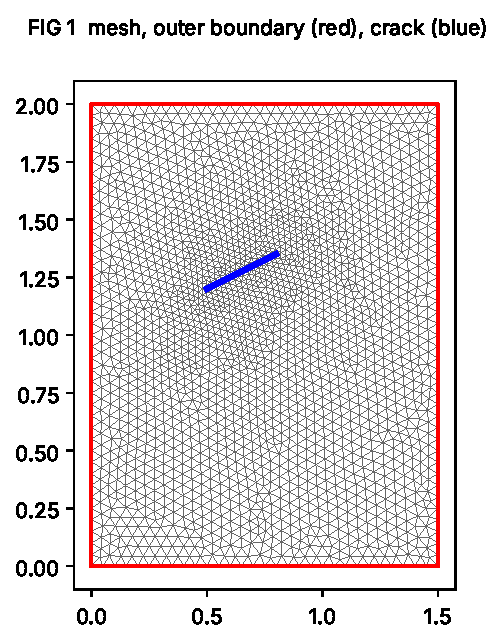
\includegraphics[height=4.6cm]{ch3/figs/python/fig1}\hfill
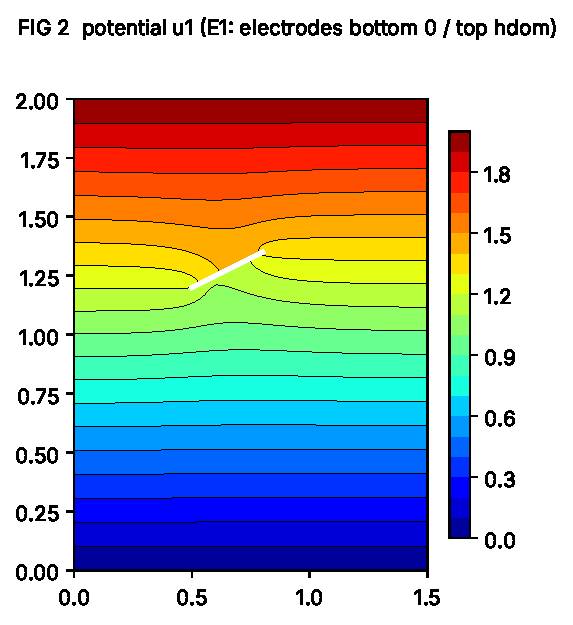
\includegraphics[height=4.6cm]{ch3/figs/python/fig2}\hfill
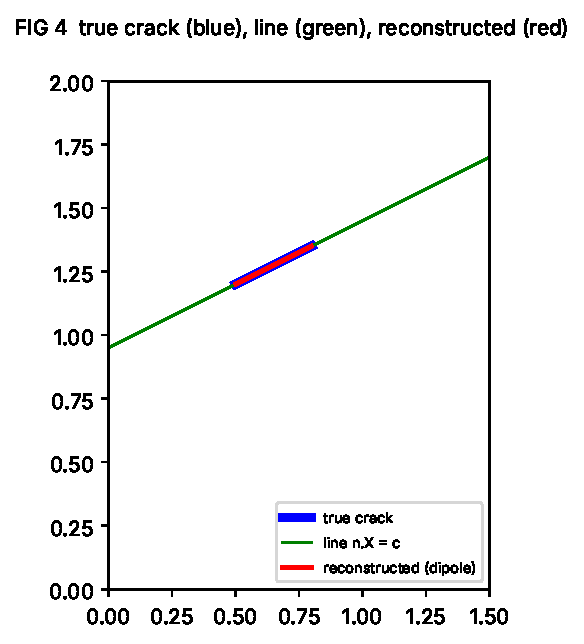
\includegraphics[height=4.2cm]{ch3/figs/python/fig4}
\end{center}
\textbf{FIG 1 -- mesh.} Red: outer boundary, where the data are measured;
blue: the crack, whose nodes are doubled (two lips). The mesh is refined at
the crack (size $\ell_\Gamma/15$) and has size $\ell/30$ elsewhere.
\textbf{FIG 2 -- potential $u_1$.} Far from the crack the isolines are
straight (the field $(0,1)$); near the crack they are bent and crowd at the
tips, since no current crosses it. \textbf{FIG 4 -- identified crack.} Blue:
true crack; green: line $\vn\cdot\vect X=c$ (Block 6); red: reconstructed
segment $\vx_0+c\vn+(s_0\pm a_{\rm dip})\vt$ (Block 7). Without noise red covers
blue.

\begin{center}
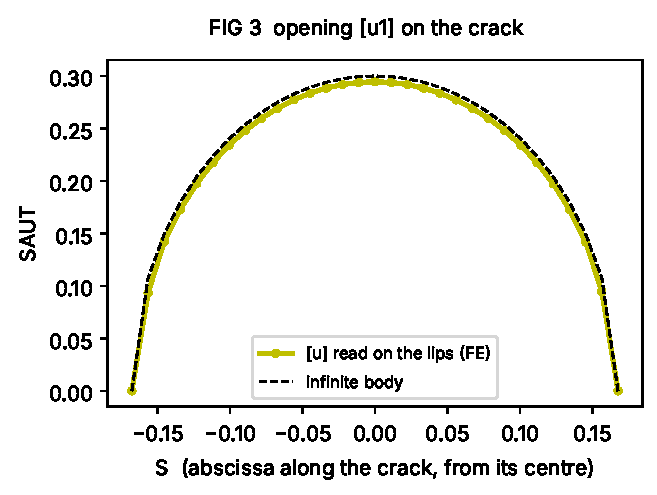
\includegraphics[width=0.32\textwidth]{ch3/figs/python/fig3}\hfill
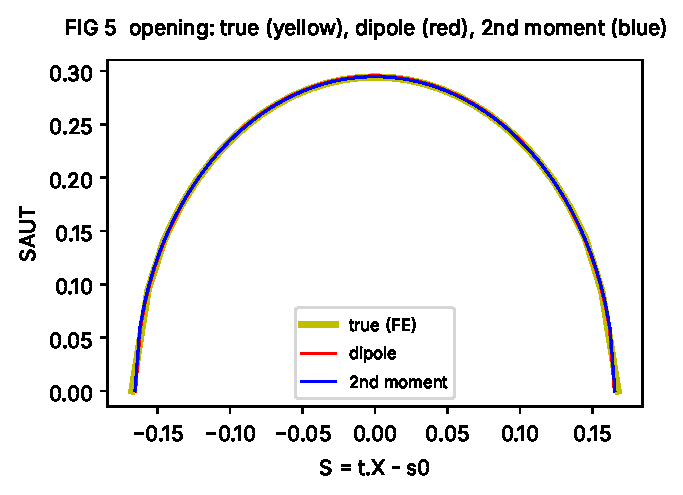
\includegraphics[width=0.32\textwidth]{ch3/figs/python/fig5}\hfill
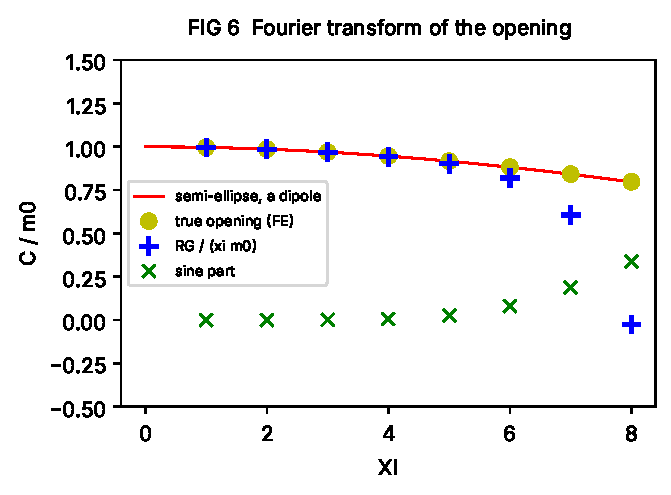
\includegraphics[width=0.32\textwidth]{ch3/figs/python/fig6}
\end{center}
\textbf{FIG 3 -- opening $\jump{u_1}$} read on the doubled nodes, against the
infinite-body opening $2E_n\sqrt{a^2-s^2}$ (dashed), slightly larger.
\textbf{FIG 5 -- opening and reconstructions.} Yellow: true opening;
red: semi-ellipse of area $m_0$ and half-length $a_{\rm dip}$; blue: the same
with $a_{\rm mom}$ (drawn only if $\mu_2>0$). Without noise they coincide; with
noise blue moves first. \textbf{FIG 6 -- Fourier transform.} Red:
$2J_1(\xi a)/(\xi a)$ with $a=a_{\rm dip}$; yellow: $C/m_0$ of the true
opening; blue crosses: $\RG/(\xi m_0)$; green: the sine part $S/m_0$, which
should vanish. Crosses leave the curve, and green leaves $0$, from
$\xi\approx5$.

\begin{center}
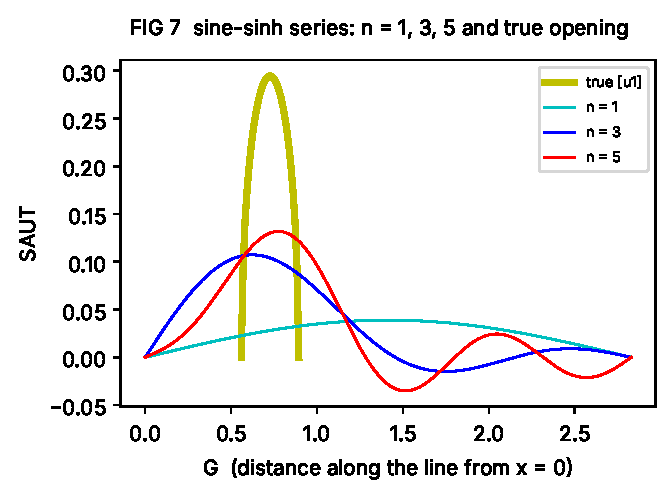
\includegraphics[width=0.32\textwidth]{ch3/figs/python/fig7}\hfill
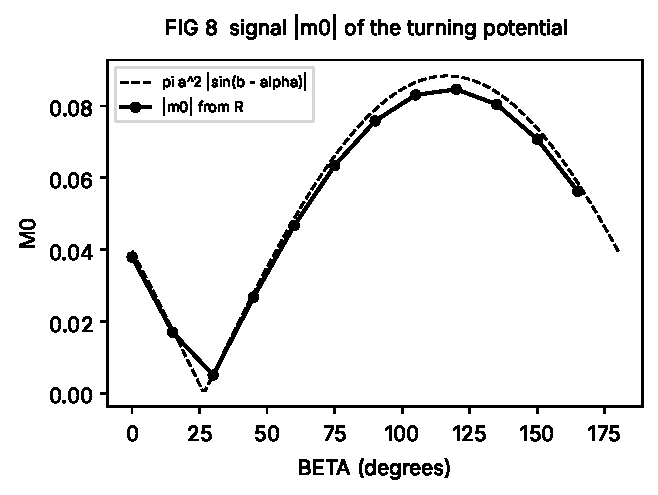
\includegraphics[width=0.32\textwidth]{ch3/figs/python/fig8}\hfill
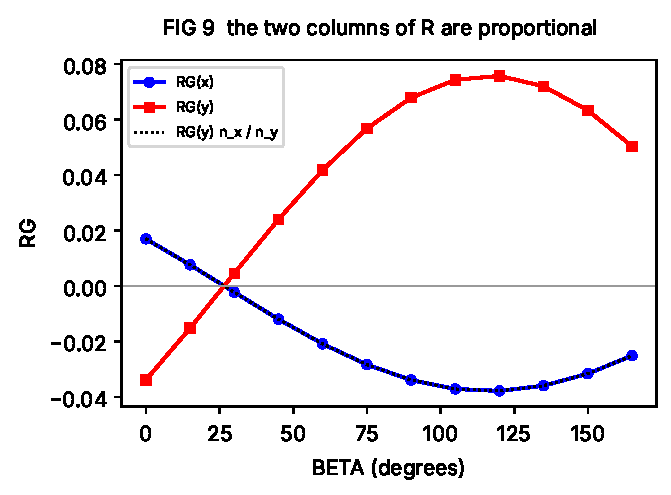
\includegraphics[width=0.32\textwidth]{ch3/figs/python/fig9}
\end{center}
\textbf{FIG 7 -- sine--sinh series.} Abscissa $g$ from the point of the line
at $x=0$, $L=\sqrt2\max(\ell,h)=2.83$; yellow: true opening; partial sums
$n=1,3,5$. The terms resolve details of size $L/n\gtrsim0.5$, larger than the
crack, and the high terms carry the discretization error.
\textbf{FIG 8 -- signal of the turning potential.} $|m_0|$ against $\beta$,
with $\pi a^2|\sin(\beta-\alpha)|$ (dashed): zero for the field parallel to
the crack ($\alpha=26.6^\circ$), largest for the normal field.
\textbf{FIG 9 -- the columns of $R$.} $\RG(X)$ and $\RG(Y)$ against $\beta$:
proportional, in the ratio $n_x/n_y$ (dotted, on top of the blue curve).

\guidesec{5\quad Reference values}
Python and FEniCS (same gmsh mesh: 4242 triangles, 8654 nodes, P2) at
\texttt{eps = 0}. True crack: $\vn=(-0.4472,0.8944)$, $c=0.2907$, length
$0.3354$, centre $(0.65,1.275)$. Cast3M, on its own mesh, should agree to
about two digits.
\begin{center}\small
\renewcommand{\arraystretch}{1.1}
\begin{tabular}{>{\sffamily}l l l}
\toprule
block & message & value\\
\midrule
4 & \texttt{int [u] on the lips} (infinite body) & 0.07641 (0.07903)\\
5 & \texttt{RG(1)} & $\approx10^{-13}$\\
6 & \texttt{RG(x)}, \texttt{RG(y)} & $-0.03427$, $0.06855$\\
6 & \texttt{normal n}, \texttt{angle error} & $(-0.4472, 0.8944)$, $0.0000^\circ$\\
6 & \texttt{line c} & 0.2907\\
7 & \texttt{m0}, \texttt{s0}, \texttt{mu2}, \texttt{E\_n} & 0.07664, $-0.0336$, 0.006855, 0.8944\\
7 & \texttt{length (2nd moment)}, \texttt{(dipole)} & 0.3312, 0.3303 (tip error 0.0026)\\
8 & $C/m_0$ at $\xi=1,2,3,4$ & 0.9966, 0.9864, 0.9691, 0.9428\\
8 & \texttt{length (Fourier, xi = 2)} & 0.3306\\
8 & sine--sinh \texttt{RG\_k}, $k=1..5$ & $-0.0551$, $-0.0753$, $-0.0487$, 0.0051, 0.0467\\
9 & singular values of $R$ & 0.20767, $\approx10^{-13}$\\
9 & $|m_0|$ min / max & 0.0051 at $30^\circ$ / 0.0846 at $120^\circ$\\
9 & virtual field $\vd_{\rm v}$, $c$, length & $(-1.0954, 2.1909)$, 0.2907, 0.3285\\
\bottomrule
\end{tabular}
\end{center}
With noise each run draws new numbers (Python and FEniCS: change
\texttt{seed}). Over 200 draws for E1: at $\texttt{eps}=10^{-3}$, dipole length
$0.330\pm0.001$, second-moment length $0.325\pm0.078$ (3 failures,
$\mu_2\le0$); at $10^{-2}$, $0.331\pm0.010$ and $0.61\pm0.25$ (81 failures).

\clearpage
%======================================================================
%  Guide: rg_session.dgibi (Cast3M)
%======================================================================
\sessiontitle{Guide 1 -- Cast3M: \texttt{rg\_session.dgibi}}
  {Blocks, figures and how to run them. Built on
   \texttt{crack\_rg\_extension.dgibi} (version 3, Cast3M 2026).}

\untested{Status: this file has not been run with Cast3M yet. It uses the
constructions of crack\_rg\_extension.dgibi (run with Cast3M 2026) and the
rules of its header; the values of Section 5 of the common part are the
references it must reproduce to about two digits.}

\guidesec{1\quad Running the file}
\begin{enumerate}[itemsep=1pt]
\item Put \texttt{rg\_session.dgibi} in a working folder and open a terminal
there.
\item Run it with your Cast3M launcher (\texttt{castem26}, \texttt{castem}, \dots),
keeping a log:
\begin{lstlisting}[style=shstyle]
cd ~/work/rg
castem26 rg_session.dgibi 2>&1 | tee run.log
\end{lstlisting}
\item With \texttt{graph = vrai}, each \op{trac}/\op{dess} opens a window and the
run waits there; close it (or use the continue control of your version) to
go to the next figure. The messages \texttt{FIG k : ...} are printed just
before.
\item To get files instead of windows, uncomment \texttt{opti trac psc;} at
the top: the plots go to a PostScript file (convert with \texttt{ps2pdf}).
\item For a run without graphics, \texttt{graph = faux;}. The run takes a few
seconds.
\end{enumerate}

\guidesec{2\quad Parameters (Block 0)}
\begin{center}\small
\begin{tabular}{>{\ttfamily}l l p{8cm}}
\toprule
\rmfamily name & default & meaning\\
\midrule
ldom, hdom & 1.5, 2. & width and height of the rectangle\\
nelem & 30 & elements per outer side ($\texttt{nelem}/2$ on the crack and the cut lines)\\
xpa ypa xpb ypb & crack tips & the true crack $A$--$B$ (mesh and errors only)\\
eps & 0. & relative noise on the measured values (0. = exact data)\\
nxi, xiest & 8, 2. & Fourier fields $\xi=1\dots\texttt{nxi}$; $\xi$ of the length estimate\\
nsine & 5 & number of sine--sinh terms\\
nbeta & 12 & turning potential: angles $0,\,180/\texttt{nbeta},\dots$ degrees\\
graph & vrai & draw the figures\\
\bottomrule
\end{tabular}
\end{center}
Recipes: \textbf{check the installation} with \texttt{eps = 0.}: angle error
$<10^{-2}$ degree, $c\approx0.291$, lengths $\approx0.33$. \textbf{Noise}:
\texttt{eps = 0.001;} or \texttt{0.01;}, several runs: \op{bruit} draws a new
realisation each time. \textbf{Mesh}: \texttt{nelem = 16} or \texttt{60}; Steps
1--2 do not change (exact identity), the Fourier and sine--sinh values do.
\textbf{Other cracks}: change \texttt{xpa \dots\ ypb}, keeping $A$ closer to
$p_1=(0,0)$ than $B$ and both tips inside the domain.

\guidesec{3\quad The blocks}
\block{Block 1 -- Geometry and mesh.} The construction of
\texttt{crack\_rg\_extension.dgibi}: the lips \texttt{dplus} and \texttt{dmoins}
are two \op{droite} with the same end points, and the domain is the union of
\texttt{smoins} and \texttt{splus}, meshed by \op{surf} on either side of the cut
$p_1$--$A$--$B$--$p_3$. The crack nodes are therefore doubled, except at the
tips. \texttt{cdom} is the outer boundary.

\block{Block 2 -- Model.} Thermal model, \texttt{K = 1}, \texttt{KK = cond mo ma}.
Centred coordinates \texttt{xr}, \texttt{yr}; the absolute \texttt{xx}, \texttt{yy}
are kept for Block 8b. FIG~1.

\block{Block 3 -- Procedures.} \texttt{rgap ub qb v kk} returns
$\RG_h(v)=\op{xty}(u_b,(Kv)_b)-\op{xty}(q_b,v_b)$; the test field is renamed
to the component \texttt{T} (\op{exco}) and reduced to the boundary nodes
(\op{redu}) before \op{xty}. \texttt{mesbr u kk cd dmu dmq epu epq} returns the
boundary potential (\texttt{T}) and flux (\texttt{Q} $=$ \texttt{KK * u}) with the
noise of \op{bruit} on the measured parts \texttt{dmu}, \texttt{dmq} only.
\texttt{ztrap ls lv} integrates a list by trapezoids (it avoids \op{intg} on an
evolution).

\block{Block 4 -- Experiment E1.} \op{bloq} on \texttt{d12}, \texttt{d34}, \op{depi}
$h$ on the top, \op{reso}. FIG~2. The opening is read with
\texttt{evol 'CHPO'} on the two lips (same nodes, same order); its integral
\texttt{mtru} and the infinite-body curve are FIG~3.

\block{Block 5 -- Measurement.} $u$ measured on the vertical sides without the
corners (\texttt{pver}), flux on the electrodes (\texttt{dhor}). $\RG(1)$ with the
field of ones \texttt{exp (0. * xr)} (no \op{masq}).

\block{Block 6 -- Normal and line.} \texttt{rx}, \texttt{ry}, $m_0$, $\vn$,
$\vt=(-n_y,n_x)$, then $c$ with \texttt{v2}. The angle error is \op{acos}
of $|\vn\cdot\vn_{\rm true}|$, in degrees.

\block{Block 7 -- Moments and dipole.} \texttt{eta}, \texttt{ss*eta},
\texttt{v3 = sp*sp*eta - eta**3/3}; \texttt{amom} is set to 0 when $\mu_2\le0$.
$E_n=\vE\cdot\vn$ with $\vE=(0,1)$. The tips $\vx_0+c\vn+(s_0\pm a_{\rm dip})\vt$
give FIG~4; the semi-ellipses of area $m_0$ give FIG~5.

\block{Block 8 -- Fourier and sine--sinh.} (a) For $\xi=1\dots\texttt{nxi}$:
\texttt{egro = exp (xi * eta)}, \texttt{vc} and \texttt{vs} with \op{cos}/\op{sin}
of \texttt{r2d * xi * sp} (degrees); the true $C(\xi)$ is integrated on the lips
with \texttt{ztrap}. The length uses the closed-form root of
$x^4/192-x^2/8+1-\rho=0$. FIG~6, with $2J_1(x)/x$ by its series.
(b) The method of the original procedure with its formula corrected:
$t$ oriented towards $x>0$, abscissa $g$ from the point of the line at $x=0$,
\texttt{LL} $=\sqrt2\max(\ell,h)$, coefficients $2\RG(v_k)/L$. FIG~7.

\block{Block 9 -- Turning potential.} \texttt{bord = bloq 'T' cdom}; the
boundary values of \texttt{xr}, \texttt{yr} renamed \texttt{T} are imposed with
\op{depi}: two solves \texttt{upx}, \texttt{upy}. For each angle,
$u_\beta=\cos\beta\,u_x+\sin\beta\,u_y$, flux measured with noise, data stored
in the tables \texttt{tub}, \texttt{tqb} (indexed by integers: no table of
tables), rows of $R$ in \texttt{lrx}, \texttt{lry}. $R^\top R$ is the $2\times2$
matrix \texttt{[saa sab; sab sdd]}: its eigenvalues in closed form, its first
eigenvector is the normal (no \op{atg}). Weights, virtual field and the
virtual experiment follow. FIG~8 and FIG~9.

\guidesec{4\quad The figures}
\begin{center}\small
\begin{tabular}{>{\sffamily}l l l}
\toprule
figure & block & gibiane\\
\midrule
FIG 1 & 2 & \texttt{trac (dom et (cdom coul roug) et (lips coul bleu))}\\
FIG 2 & 4 & \texttt{trac dom u1 (cont dom)}\\
FIG 3 & 4 & \texttt{dess (evj et evi)}, evolutions \texttt{evol manu 'S' ... 'SAUT'}\\
FIG 4 & 7 & \texttt{trac (cdom et dplus et dfis et lfis)}, colours blue, green, red\\
FIG 5 & 7 & \texttt{dess evtot}: yellow, red, blue\\
FIG 6 & 8 & \texttt{dess ev6 'YBOR' -0.5 1.5}: red, yellow, blue, green\\
FIG 7 & 8 & \texttt{dess (evg et es1 et es3 et es5)}\\
FIG 8, 9 & 9 & \texttt{dess ev8}, \texttt{dess ev9}\\
\bottomrule
\end{tabular}
\end{center}
They show what the figures of the common part show (Section 4), in the
style of Cast3M. With noise, the details change at each run.

\guidesec{5\quad The printed messages}
Each block prints a line starting with \texttt{BLOCK k}, with the values of
the table of the common part (Section 5); the sine--sinh coefficients are
printed with \op{list}. Signs: $\vn$ is oriented so that $m_0>0$, and $c$,
$s_0$, $E_n$ change sign with it. The mesh of \op{surf} is less regular than
the gmsh mesh: Steps 1--2 are exact on both, the lengths agree to about
$0.005$, and the Fourier values may leave the true ones at a lower $\xi$
(watch $S(\xi)/m_0$).

\guidesec{6\quad Gibiane pitfalls}
\begin{itemize}[itemsep=1pt]
\item \textbf{Operator names.} Gibiane recognises operators by their first
four letters: a name such as \texttt{mesu} (\op{mesure}), \texttt{tres}
(\op{tresca}) or \texttt{et} breaks later instructions. Hence \texttt{mesbr},
\texttt{ztrap}, \texttt{egro}, \texttt{dsc}, \texttt{tvx}.
\item \textbf{Case.} Gibiane ignores case: \texttt{XX} and \texttt{xx} are the
same name.
\item \textbf{Knock-on errors.} When an instruction fails, its result is not
created and the error appears later, where the object is used. Look for the
\emph{first} \texttt{ERREUR} in the log (\texttt{opti echo 1;} prints each
instruction).
\item \textbf{Dots and digits.} \texttt{w.1} or \texttt{t1.1.'UB'} can be read as
real numbers: write table indices with spaces, \texttt{tub . k}.
\item \textbf{Components.} Products and sums of \texttt{CHPOINT}s combine the
components of the same name: \op{exco} \texttt{'SCAL' 'T'} renames a test
field so that it meets the potential, and \op{xty} is given the component
names explicitly.
\item \textbf{Degrees.} \op{sin}, \op{cos} and \op{acos} work in degrees:
\texttt{r2d = 180/pi}.
\item \textbf{Procedure arguments} are matched by type, in order within each
type; several results are returned in the order of \op{finproc}.
\item \textbf{Forbidden here} (author's rules, Cast3M 2026): \op{masq},
\op{atg}, tables of tables built in one chain, lines longer than 72 columns.
\end{itemize}

\guidesec{7\quad Listing of \texttt{rg\_session.dgibi}}
\lstinputlisting[style=gibstyle]{cast3m/ch3/rg_session.dgibi}

\clearpage
%======================================================================
%  Guide: rg_session_fenics.py (FEniCS / DOLFINx)
%======================================================================
\sessiontitle{Guide 2 -- FEniCS: \texttt{rg\_session\_fenics.py}}
  {Blocks, figures and how to run them. Built on
   \texttt{reciprocity\_gap\_crack.py} (DOLFINx + gmsh).}

\untested{Status: not run with DOLFINx yet. Blocks 1 and 4--9 were run
(gmsh mesh, then the same arrays assembled with scikit-fem: this is the
Python file of Guide 3); Blocks 2--3 use the DOLFINx calls of
reciprocity\_gap\_crack.py. The values of Section 5 of the common part are
the references.}

\guidesec{1\quad Running the file}
\begin{enumerate}[itemsep=1pt]
\item Install DOLFINx 0.8--0.10 with gmsh (conda is the simplest route):
\begin{lstlisting}[style=shstyle]
conda create -n fenicsx -c conda-forge fenics-dolfinx mpich gmsh python-gmsh scipy matplotlib
conda activate fenicsx
\end{lstlisting}
\item Run it in serial, with the noise level and the folder of the figures
as optional arguments:
\begin{lstlisting}[style=shstyle]
python3 rg_session_fenics.py              # eps = 0, figures in .
python3 rg_session_fenics.py 0.01 figs    # eps = 0.01, figures in figs/
RG_NELEM=60 python3 rg_session_fenics.py  # finer mesh
\end{lstlisting}
\item The figures are written to \texttt{fig1.pdf} \dots\ \texttt{fig9.pdf}; the
messages \texttt{FIG k : ...} are printed when each is saved. The run takes a
few seconds.
\end{enumerate}

\guidesec{2\quad Parameters (Block 0)}
\begin{center}\small
\begin{tabular}{>{\ttfamily}l l p{8cm}}
\toprule
\rmfamily name & default & meaning\\
\midrule
ldom, hdom & 1.5, 2.0 & width and height of the rectangle\\
nelem & 30 & mesh size $\ell/\texttt{nelem}$, $\ell_\Gamma/(\texttt{nelem}/2)$ on the crack (\texttt{RG\_NELEM})\\
A, B & crack tips & the true crack (mesh and errors only)\\
eps & 0 & relative noise on the measured values (first argument)\\
seed & 1 & seed of the noise: change it to draw again\\
nxi, xiest & 8, 2.0 & Fourier fields $\xi=1\dots\texttt{nxi}$; $\xi$ of the length estimate\\
nsine & 5 & number of sine--sinh terms\\
nbeta & 12 & turning potential: angles $0,15,\dots,165$ degrees\\
outdir & . & folder of the figures (second argument)\\
\bottomrule
\end{tabular}
\end{center}

\guidesec{3\quad The blocks}
\block{Block 1 -- Geometry and mesh.} As in \texttt{replica.py}: gmsh
rectangle, the crack line embedded (\texttt{mesh.embed}), size
\texttt{Mesh.MeshSizeMax} $=\ell/30$ and $\ell_\Gamma/15$ at the tips. The gmsh
plugin \texttt{Crack} then duplicates the nodes of the crack (not the tips).
\texttt{gmshio.model\_to\_mesh} gives the DOLFINx mesh (the module is
\texttt{dolfinx.io.gmsh} from 0.10).

\block{Block 2 -- Model.} \texttt{functionspace(msh, ("Lagrange", 2))}: P2,
the TRI6 of Cast3M. The matrix $\mat K$ is assembled \emph{without} boundary
conditions and converted to SciPy (\texttt{fem.assemble\_matrix(a).to\_scipy()}):
$q=\mat Ku$ are then the nodal fluxes, as \texttt{KK * u} in Cast3M. The node
coordinates are \texttt{V.tabulate\_dof\_coordinates()}; \texttt{upnode} marks
the nodes of the cells on the side of $\vn$, which tells the lips apart.
FIG~1 uses the vertices of the cells (P1 space).

\block{Block 3 -- Procedures.} \texttt{rgap}, \texttt{measure}, \texttt{opening}
work on NumPy arrays and are the same as in Python. \texttt{dirichlet(mask,
values)} solves with \texttt{LinearProblem} and \texttt{dirichletbc} on the
nodes of \texttt{mask} (direct LU solver); the other boundary nodes and the
lips get the natural zero flux.

\block{Blocks 4--9.} The same text as in the Python file (Guide~3): from Block 4
on, the identification needs only the boundary values, the matrix $\mat K$
and the node coordinates. E1 is \texttt{dirichlet(bot | top, y)}; the turning
potential uses \texttt{dirichlet(outer, X)} and \texttt{dirichlet(outer, Y)}.
$R$ is decomposed with \texttt{numpy.linalg.svd}.

\guidesec{4\quad The figures}
\begin{center}\small
\begin{tabular}{>{\sffamily}l l l}
\toprule
figure & block & matplotlib\\
\midrule
FIG 1 & 2 & \texttt{triplot} of the vertices, boundary and crack\\
FIG 2 & 4 & \texttt{tricontourf} of $u_1$ at the vertices\\
FIG 3 & 4 & opening on the lips and infinite-body curve\\
FIG 4, 5 & 7 & identified line and segment; semi-ellipses\\
FIG 6, 7 & 8 & $C/m_0$, $S/m_0$ against $\xi$; sine--sinh sums\\
FIG 8, 9 & 9 & $|m_0|$ and the columns of $R$ against $\beta$\\
\bottomrule
\end{tabular}
\end{center}
The mesh is the gmsh mesh of the Python file: the figures are those of the
common part (Section 4).

\guidesec{5\quad The printed messages}
One line per block, \texttt{BLOCK k ...}, with the values of Section 5 of the
common part (same mesh, same element: the same numbers up to round-off).
Signs: $\vn$ is oriented so that $m_0>0$.

\guidesec{6\quad FEniCS pitfalls}
\begin{itemize}[itemsep=1pt]
\item \textbf{The lips are boundary facets.} After the \texttt{Crack} plugin,
\texttt{locate\_entities\_boundary} also returns the facets of the lips. Here
the outer boundary is selected by coordinates (\texttt{outer}), never by
``boundary facet''.
\item \textbf{Reactions.} \texttt{LinearProblem} with Dirichlet conditions
modifies the rows of the constrained nodes; the fluxes $\mat Ku$ need the
matrix assembled without conditions (Block 2).
\item \textbf{Serial only.} With MPI, the arrays are distributed and the
indices of \texttt{tabulate\_dof\_coordinates} are local; run with one
process.
\item \textbf{Versions.} \texttt{dolfinx.io.gmshio} became \texttt{dolfinx.io.gmsh}
in 0.10, and \texttt{LinearProblem} needs \texttt{petsc\_options\_prefix} there;
the file tries both.
\item \textbf{Mesh regularity.} The Fourier and sine--sinh fields are not
polynomials: their gaps carry a discretization error that depends on the size
\emph{and} the regularity of the mesh (sheet, question f.4).
\end{itemize}

\guidesec{7\quad Listing of \texttt{rg\_session\_fenics.py}}
\lstinputlisting[style=pystyle,lastline=231]{fenics/ch3/rg_session_fenics.py}
\noindent\emph{Blocks 4--9: the same text as in the Python file (Guide~3,
Section~7).}

\clearpage
%======================================================================
%  Guide: rg_session.py (Python, scikit-fem + gmsh)
%======================================================================
\sessiontitle{Guide 3 -- Python: \texttt{rg\_session.py}}
  {Blocks, figures and how to run them. Built on the replica
   \texttt{replica.py} (gmsh + scikit-fem).}

\guidesec{1\quad Running the file}
\begin{enumerate}[itemsep=1pt]
\item Install the packages (any Python $\ge3.9$):
\begin{lstlisting}[style=shstyle]
pip install numpy scipy matplotlib scikit-fem gmsh
\end{lstlisting}
On Linux, the \texttt{gmsh} wheel needs the system libraries of OpenGL
(\texttt{libglu1-mesa}, \texttt{libxcursor1}, \texttt{libxinerama1},
\texttt{libxft2}).
\item Run it, with the noise level and the folder of the figures as optional
arguments:
\begin{lstlisting}[style=shstyle]
python3 rg_session.py              # eps = 0, figures in .
python3 rg_session.py 0.01 figs    # eps = 0.01, figures in figs/
RG_NELEM=60 python3 rg_session.py  # finer mesh
\end{lstlisting}
\item The figures are written to \texttt{fig1.pdf} \dots\ \texttt{fig9.pdf}; the
messages \texttt{FIG k : ...} are printed when each is saved. The run takes
about three seconds.
\end{enumerate}

\guidesec{2\quad Parameters (Block 0)}
\begin{center}\small
\begin{tabular}{>{\ttfamily}l l p{8cm}}
\toprule
\rmfamily name & default & meaning\\
\midrule
ldom, hdom & 1.5, 2.0 & width and height of the rectangle\\
nelem & 30 & mesh size $\ell/\texttt{nelem}$, $\ell_\Gamma/(\texttt{nelem}/2)$ on the crack (\texttt{RG\_NELEM})\\
A, B & crack tips & the true crack (mesh and errors only)\\
eps & 0 & relative noise on the measured values (first argument)\\
seed & 1 & seed of the noise: change it to draw again\\
nxi, xiest & 8, 2.0 & Fourier fields $\xi=1\dots\texttt{nxi}$; $\xi$ of the length estimate\\
nsine & 5 & number of sine--sinh terms\\
nbeta & 12 & turning potential: angles $0,15,\dots,165$ degrees\\
outdir & . & folder of the figures (second argument)\\
\bottomrule
\end{tabular}
\end{center}

\guidesec{3\quad The blocks}
\block{Block 1 -- Geometry and mesh.} The gmsh model of \texttt{replica.py}
(and of the FEniCS file): rectangle, embedded crack, \texttt{Crack} plugin.
The nodes and triangles are read back from gmsh and give a scikit-fem
\texttt{MeshTri}; nodes not used by a triangle are dropped.

\block{Block 2 -- Model.} \texttt{Basis(mesh, ElementTriP2())} and the
stiffness matrix of $\nabla u\cdot\nabla v$, without boundary conditions (nodal
fluxes $q=\mat Ku$). \texttt{basis.doflocs} gives the node coordinates;
\texttt{upnode} the nodes of the cells on the side of $\vn$. FIG~1.

\block{Block 3 -- Procedures.} \texttt{rgap(ub, qb, v)} is
$\sum_{\partial\Omega}u(\mat Kv)-qv$; \texttt{measure} adds the noise to the
measured values; \texttt{opening(u)} pairs the doubled nodes of the crack by
their abscissa and returns $u^+-u^-$; \texttt{dirichlet(mask, values)} solves
with \texttt{condense} and \texttt{solve}.

\block{Block 4 -- Experiment E1.} \texttt{u1 = dirichlet(bot | top, y)}. FIG~2
and FIG~3 (opening, its integral, the infinite-body curve).

\block{Block 5 -- Measurement.} $u$ on the vertical sides without corners,
$q$ on the electrodes; $\RG(1)$.

\block{Blocks 6--7.} Normal, line, moments, lengths, tips; FIG~4 and FIG~5.

\block{Block 8.} (a) Fourier fields, $C/m_0$ and $S/m_0$ against the true
$C/m_0$ of the opening on the lips, length from $\xi=\texttt{xiest}$; FIG~6.
(b) Sine--sinh series as in Cast3M; FIG~7.

\block{Block 9.} Two solves \texttt{ux}, \texttt{uy}; for each angle the noisy
flux, the row of $R$; \texttt{numpy.linalg.svd(R)}, the normal, the weights,
the virtual experiment; FIG~8 and FIG~9.

\guidesec{4\quad The figures}
Those of the common part (Section 4), which were produced by this file:
\texttt{triplot} (FIG~1), \texttt{tricontourf} (FIG~2), line plots (FIG~3, 5--9),
the geometry (FIG~4).

\guidesec{5\quad The printed messages}
One line per block, \texttt{BLOCK k ...}, with the values of Section 5 of the
common part. Signs: $\vn$ is oriented so that $m_0>0$. With
\texttt{eps = 0.01} and \texttt{seed = 1}, for instance: angle error
$4.36^\circ$ (E1) against $0.64^\circ$ (the twelve turning experiments), dipole
length $0.331$, second moment failed ($\mu_2<0$).

\guidesec{6\quad Python pitfalls}
\begin{itemize}[itemsep=1pt]
\item \textbf{Nodes of P2.} \texttt{basis.doflocs} lists the vertices first,
then the midpoints of the edges; the colour plots use only the vertices.
\item \textbf{The lips.} After the \texttt{Crack} plugin, two nodes have the same
coordinates; any search by coordinates must keep both (\texttt{opening}) and
tell them apart by the cells they belong to (\texttt{upnode}).
\item \textbf{Unused gmsh nodes.} gmsh keeps the nodes of the
one-dimensional crack elements; they belong to no triangle and must be
dropped, or the matrix is singular.
\item \textbf{Noise and seed.} The generator is created once
(\texttt{default\_rng(seed)}): Blocks 5 and 9 draw from it in turn.
\end{itemize}

\guidesec{7\quad Listing of \texttt{rg\_session.py}}
\lstinputlisting[style=pystyle]{python/examples/ch3/rg_session.py}

\endgroup

%---- 3. the session sheet with the answers ------------------------------
\clearpage
\answerstrue
\setcounter{spart}{0}
%======================================================================
%  Session sheet, Chapter 3 (reciprocity gap). Printed twice by
%  session_ch3.tex: without and with the answers. No \label here.
%======================================================================
\ifanswers
\sessiontitle{Chapter 3 -- Reciprocity: session sheet with answers}
  {Answers. Numbers from the Python and FEniCS codes (same gmsh mesh,
   $30$ divisions, P2); Cast3M meshes differently and agrees to about
   two digits.}
\else
\sessiontitle{Chapter 3 -- Reciprocity: session sheet}
  {Notes: Chapter~\ref{B-ch:rg}, Sections~\ref{B-sec:rg-gap}--\ref{B-sec:rg-num}.
   Codes: \texttt{rg\_session} in Cast3M, FEniCS or Python (guides at the
   end of this document).}
\fi

\paragraph{The setting.} A conducting rectangle $\Omega=(0,\ell)\times(0,h)$,
$\ell=1.5$, $h=2$, with conductivity $1$, contains an insulating crack
$\Gamma$, the segment from $A=(0.5,\,1.2)$ to $B=(0.8,\,1.35)$
(Figure~a). The crack is unknown to the identification; $A$ and $B$ only
build the mesh and measure the errors. Coordinates are centred,
$\vect X=\vx-\vx_0$, $\vx_0=(0.75,\,1)$. Two kinds of experiments are used.
\begin{itemize}[itemsep=1pt,topsep=2pt]
\item \textbf{E1, electrodes.} $u=0$ on the bottom, $u=h$ on the top, zero
flux on the vertical sides. The potential is measured on the vertical
sides, the flux (current) on the electrodes.
\item \textbf{Turning potential.} $u=\vd_\beta\cdot\vect X$ on the whole
boundary, $\vd_\beta=(\cos\beta,\sin\beta)$, $\beta=0^\circ,15^\circ,
\dots,165^\circ$. Only the flux is measured (Figure~b).
\end{itemize}

\begin{center}
\begin{tikzpicture}[scale=1.3,>=Stealth]
  % (a) experiment E1
  \begin{scope}
  \fill[gray!8] (0,0) rectangle (1.5,2);
  \draw[cu,line width=2pt] (0,0) -- (1.5,0);
  \draw[cu,line width=2pt] (0,2) -- (1.5,2);
  \draw[cphi,line width=1.2pt] (0,0) -- (0,2);
  \draw[cphi,line width=1.2pt] (1.5,0) -- (1.5,2);
  \draw[very thick] (0.5,1.2) -- (0.8,1.35);
  \fill (0.5,1.2) circle (0.8pt) node[left,font=\scriptsize] {$A$};
  \fill (0.8,1.35) circle (0.8pt) node[right,font=\scriptsize] {$B$};
  \draw[->] (0.65,1.275) -- ++(-0.13,0.26) node[above,font=\scriptsize] {$\vn$};
  \node[font=\scriptsize,cu] at (0.75,-0.17) {$u=0$, flux measured};
  \node[font=\scriptsize,cu] at (0.75,2.17) {$u=h$, flux measured};
  \node[font=\scriptsize,cphi,rotate=90] at (-0.22,1) {$\partial_\nu u=0$, $u$ measured};
  \node[font=\scriptsize,cphi,rotate=90] at (1.72,1) {$\partial_\nu u=0$, $u$ measured};
  \fill (0.75,1) circle (0.6pt) node[below,font=\scriptsize] {$\vx_0$};
  \node[font=\sffamily\small] at (0.75,-0.5) {(a) experiment E1};
  \end{scope}
  % (b) turning potential
  \begin{scope}[xshift=3.4cm]
  \fill[gray!8] (0,0) rectangle (1.5,2);
  \draw[cu,line width=2pt] (0,0) rectangle (1.5,2);
  \draw[very thick] (0.5,1.2) -- (0.8,1.35);
  \draw[->,thick] (0.75,1) -- ++(40:0.45) node[right,font=\scriptsize] {$\vd_\beta$};
  \draw (0.95,1) arc (0:40:0.2) node[midway,right,font=\scriptsize] {$\beta$};
  \draw[gray] (0.75,1) -- (1.1,1);
  \node[font=\scriptsize,cu,align=center] at (0.75,-0.22)
    {$u=\vd_\beta\cdot\vect X$ imposed,\\ flux measured};
  \node[font=\sffamily\small] at (0.75,-0.62) {(b) turning potential};
  \end{scope}
  % (c) the line and the coordinates
  \begin{scope}[xshift=6.4cm,yshift=0.2cm]
  \draw[gray] (-0.2,0.4) -- (1.9,1.45);
  \draw[very thick] (0.6,0.8) -- (1.2,1.1);
  \draw[->] (0.9,0.95) -- ++(0.36,0.18) node[right,font=\scriptsize] {$\vt$};
  \draw[->] (0.9,0.95) -- ++(-0.18,0.36) node[above,font=\scriptsize] {$\vn$};
  \fill (0,0) circle (0.8pt) node[below,font=\scriptsize] {$\vx_0$};
  \draw[dashed] (0,0) -- (-0.2,0.4) node[midway,left,font=\scriptsize] {$c$};
  \node[font=\scriptsize,align=left,anchor=west] at (-0.3,-0.5)
    {line $\vn\cdot\vect X=c$,\\ $s=\vt\cdot\vect X$,\ $\eta=\vn\cdot\vect X-c$};
  \node[font=\sffamily\small] at (0.75,-1.0) {(c) coordinates};
  \end{scope}
\end{tikzpicture}
\end{center}

\paragraph{The codes.} The three versions have the same ten blocks, and they
print and draw the same quantities: 0 parameters; 1 mesh with two lips;
2 model and centred coordinates (FIG~1); 3 procedures; 4 experiment E1 and
its opening (FIG~2--3); 5 measurement; 6 linear and quadratic adjoint
fields; 7 polynomial fields and dipole (FIG~4--5); 8 Fourier and
sine--sinh fields (FIG~6--7); 9 turning potential and the matrix of the
experiments (FIG~8--9). Questions marked \textcolor{cu}{[code]} use them;
the others are done by hand. Run first with exact data (\texttt{eps = 0}).

%======================================================================
\spart{Direct and inverse problem -- recall of the reciprocity gap}
\begin{gbox}{Recall (Notes, Sections \ref{B-sec:rg-direct}--\ref{B-sec:rg-gap})}
Direct problem: $\Delta u=0$ in $\OG$, $\partial_nu^\pm=0$ on the lips, $u$ or
$\partial_\nu u$ given on each part of $\partial\Omega$; well posed by
Lax--Milgram. Inverse problem: $u$ \emph{and} $\varphi=\partial_\nu u$ known
on $\partial\Omega$, $\Gamma$ unknown; ill-posed. For $v$ harmonic in $\Omega$:
$\displaystyle \RG(v)=\int_{\partial\Omega}(u\,\partial_\nu v-v\varphi)\dd s=\int_\Gamma\jump u\,\partial_nv\dd s$.
\end{gbox}

\q Write the direct problem of experiment E1 (equation in $\OG$, condition on
the lips, condition on each side of $\Omega$). Which boundary values are
imposed, which are measured? Why does the identification need both?
\begin{answer}
$\Delta u=0$ in $\OG=\Omega\setminus\Gamma$; $\partial_nu^\pm=0$ on the lips;
$u=0$ on $y=0$, $u=h$ on $y=h$, $\partial_\nu u=0$ on $x=0$ and $x=\ell$.
The electrodes impose $u$ and measure the current $\partial_\nu u$; the
insulated sides impose $\partial_\nu u=0$ and measure $u$. After the
experiment both $u$ and $\varphi=\partial_\nu u$ are known on the whole
boundary (complete Cauchy data). $\RG(v)$ integrates
$u\,\partial_\nu v-v\,\varphi$ over $\partial\Omega$: it needs both.
\end{answer}

\q State the weak form of the direct problem. Why are the lip conditions
natural? Which hypothesis of the Lax--Milgram lemma uses the electrodes?
\begin{answer}
Find $u\in H^1(\OG)$, $u=0$ at the bottom and $u=h$ at the top, such that
$\displaystyle \int_{\OG}\nabla u\cdot\nabla v\dd\vx=0$ for every $v\in V=\{v\in
H^1(\OG):\ v=0$ on the electrodes$\}$. Integrating by parts, the boundary
terms are $\displaystyle \int\partial_\nu u\,v$ on the sides and on both lips:
they vanish for every $v$ only if $\partial_\nu u=0$ there. Hence the zero
flux is natural, as on the insulated sides. Coercivity on $V$ follows from
the Poincar\'e--Friedrichs inequality, which needs $u$ imposed on a part
of the boundary of positive length (the electrodes), Notes
Section~\ref{B-sec:rg-direct}.
\end{answer}

\q Let $v$ be harmonic in the uncracked $\Omega$. Apply Green's second
identity in $\OG$ and show
$\displaystyle \RG(v)=\int_{\partial\Omega}(u\,\partial_\nu v-v\,\varphi)\dd s
=\int_\Gamma\jump u\,\partial_nv\dd s$, $\jump u=u^+-u^-$, $+$ on the side
of $\vn$. Watch the normals of $\OG$ on the two lips.
\begin{answer}
$\displaystyle \int_{\OG}(v\Delta u-u\Delta v)=\int_{\partial\OG}(v\,\partial_{\nu'}u
-u\,\partial_{\nu'}v)$ and the left-hand side is $0$. On $\partial\Omega$,
$\nu'=\vnu$. On $\Gamma^+$, $\nu'=-\vn$; on $\Gamma^-$, $\nu'=+\vn$. On the
lips $\partial_{\nu'}u=0$, and $v$, $\partial_nv$ are continuous across
$\Gamma$. The lips give $\displaystyle \int_\Gamma(u^+-u^-)\partial_nv$, hence
$\displaystyle 0=\int_{\partial\Omega}(v\varphi-u\,\partial_\nu v)+\int_\Gamma\jump
u\,\partial_nv$: this is the identity (Notes, eq.~\eqref{B-eq:rg-identity}).
\end{answer}

\q Show that $\RG(1)=0$, that $\RG$ does not change if $u\to u+C$, and that
$\RG(v)=0$ for every $v$ if there is no crack.
\begin{answer}
$\displaystyle \RG(1)=-\int_{\partial\Omega}\varphi=0$, the flux balance of
$\Delta u=0$ in $\OG$ (no flux through the lips).
$\displaystyle C\int_{\partial\Omega}\partial_\nu v=C\int_\Omega\Delta v=0$.
Without crack, $u$ and $v$ are harmonic in $\Omega$ and Green's identity
gives $0$: Maxwell--Betti reciprocity. The gap measures the crack.
\end{answer}

\q \emph{Discrete gap.} The codes compute
$\RG_h(v)=\sum_{i\in\partial\Omega}\bigl(u_i(\mat Kv)_i-q_iv_i\bigr)$, with
$\mat K$ the conductivity matrix of the cracked mesh and $q=\mat Ku$ the
nodal fluxes (reactions). Show that $\RG_h(v)=-\sum_{i\notin\partial\Omega}
u_i(\mat Kv)_i$. Explain why, for a harmonic polynomial $v$ of degree $\le2$
and quadratic elements, only the nodes of the lips contribute, and
$\RG_h(v)=\int_\Gamma\jump{u_h}\,\partial_nv$ exactly.
\begin{answer}
$\mat K$ is symmetric:
$\sum_{\rm all}u_i(\mat Kv)_i=\sum_{\rm all}v_i(\mat Ku)_i=\sum_{i\in
\partial\Omega}q_iv_i$, because $(\mat Ku)_i=0$ at every node where $u$ is not
imposed (inside, insulated sides, lips). Subtracting gives the formula.
A quadratic $v$ is represented exactly by P2 elements, and
$(\mat Kv)_i=\int\nabla v\cdot\nabla\phi_i=-\int\Delta v\,\phi_i+$ boundary
terms of the support of $\phi_i$. With $\Delta v=0$ this vanishes at every
interior node whose support does not touch the crack. At a node of the upper
lip the support has the lip as boundary, with outward normal $-\vn$:
$(\mat Kv)_i=-\int_{\Gamma}\partial_nv\,\phi_i$; at the lower lip the sign is
$+$. Summing,
$\RG_h(v)=\int_\Gamma(u_h^+-u_h^-)\partial_nv$, without discretization error
beyond that of $u_h$. For other $v$ (cubic, exponential) $(\mat Kv)_i\ne0$
inside, and $\RG_h$ carries an error.
\end{answer}

\qc Run Blocks 1--5 (FIG~1--3). Check $\RG(1)\approx0$. Compare
$\displaystyle \int_\Gamma\jump{u_1}$, read on the lips, with the infinite-body
value $\pi a^2E_n$ ($a$ half-length, $E_n=\vE\cdot\vn$). Why is it smaller?
\begin{answer}
$\RG(1)\approx10^{-13}$ (round-off). $\displaystyle \int\jump{u_1}=0.0764$
against $\pi a^2E_n=0.0790$, $3\%$ less. Two reasons: the opening
vanishes at the last node before each tip (the $\sqrt r$ behaviour is
poorly represented: the mesh error), and the finite body with electrodes is
not the infinite plane. FIG~3: the shape is a semi-ellipse, slightly
below the infinite-body curve.
\end{answer}

%======================================================================
\spart{Families of adjoint fields in 2D -- the plane (the normal)}
\begin{gbox}{Recall (Notes, Section \ref{B-sec:rg-rec}, Step 1)}
$\RG(\vd\cdot\vect X)=m_0\,\vd\cdot\vn$, $\displaystyle m_0=\int_\Gamma\jump u$:
$(\RG(X),\RG(Y))=m_0\vn$, sign fixed by $m_0>0$. A uniform field parallel to
the crack opens nothing: blind experiment.
\end{gbox}

\q Show that the harmonic polynomials of degree $k\ge1$ in 2D form a space of
dimension 2, spanned by $\operatorname{Re}z^k$, $\operatorname{Im}z^k$,
$z=x+\mathrm iy$. List them up to degree 3.
\begin{answer}
A homogeneous polynomial of degree $k$ has $k+1$ coefficients; its
Laplacian is homogeneous of degree $k-2$ ($k-1$ coefficients). Harmonicity
gives $k-1$ independent conditions: dimension $2$. $\operatorname{Re}z^k$,
$\operatorname{Im}z^k$ are harmonic (real and imaginary parts of a
holomorphic function) and independent. Degree 1: $x,\ y$; degree 2:
$x^2-y^2,\ 2xy$; degree 3: $x^3-3xy^2,\ 3x^2y-y^3$.
\end{answer}

\q For $v=\vd\cdot\vect X$ show $\RG(v)=m_0\,\vd\cdot\vn$, with
$\displaystyle m_0=\int_\Gamma\jump u$. Deduce $\vn$ and $m_0$ from $\RG(X)$
and $\RG(Y)$. Is the sign of $\vn$ determined?
\begin{answer}
$\partial_nv=\vd\cdot\vn$ is constant on $\Gamma$:
$\RG(v)=\vd\cdot\vn\int\jump u$. Hence $(\RG(X),\RG(Y))=m_0\vn$,
$m_0=|(\RG(X),\RG(Y))|$, $\vn=(\RG(X),\RG(Y))/m_0$. Exchanging the lips
changes $\vn$ and $\jump u$ together: the sign is fixed by the
convention $m_0>0$.
\end{answer}

\q One measures $\RG(X)=-0.0343$, $\RG(Y)=0.0686$. Give $m_0$, $\vn$, the
angle of the crack with the $x$ axis, and the tangent $\vt$ with $(\vt,\vn)$
direct.
\begin{answer}
$m_0=\sqrt{0.0343^2+0.0686^2}=0.0767$, $\vn=(-0.447,\,0.894)$. The crack is
normal to $\vn$: $\vt=(n_2,-n_1)=(0.894,\,0.447)$, angle $\arctan(0.5)=
26.6^\circ$. (Codes: $0.07664$, $(-0.4472,0.8944)$: exact.)
\end{answer}

\q \emph{Blind experiment.} For a uniform field $\vE=(\cos\beta,\sin\beta)$,
for which $\beta$ is the crack invisible? Is E1 blind? Is the field
$(1,0)$ blind?
\begin{answer}
$m_0=|\tM|\,\vE\cdot\vn$ vanishes when $\vE\perp\vn$, i.e.\ $\vE$ parallel to
the crack: $\beta=26.6^\circ$ (mod $180^\circ$). E1 ($\vE=(0,1)$,
$E_n=0.894$) and $(1,0)$ ($|E_n|=0.447$) are not blind; E1 gives the
larger signal.
\end{answer}

\qc Run Block 6. Compare $\vn$ with the true normal; repeat with
\texttt{eps = 0.001} and \texttt{0.01}. Why is the normal exact without
noise, on a coarse mesh?
\begin{answer}
Exact data: $\vn=(-0.4472,0.8944)$, angle error $0.0000^\circ$: $X,Y$ are
of degree 1 (a.5). Over 200 draws the mean angle error is $0.24^\circ$ at
$10^{-3}$ and $2.4^\circ$ at $10^{-2}$: proportional to the noise.
\end{answer}

%======================================================================
\spart{Position -- the line of the crack}
\begin{gbox}{Recall (Step 2; 2D form, Section \ref{B-sec:rg-num})}
$v_2=(\vn\cdot\vect X)^2-(\vt\cdot\vect X)^2$, $\partial_nv_2=2c$ on the line,
$c=\RG(v_2)/\bigl(2\RG(\vn\cdot\vect X)\bigr)$.
\end{gbox}

\q Show that $v_2=(\vn\cdot\vect X)^2-(\vt\cdot\vect X)^2$ is harmonic, that
$\partial_nv_2=2c$ on the line $\vn\cdot\vect X=c$, and that
$c=\RG(v_2)/(2\RG(\vn\cdot\vect X))$. Why is it enough to know $\vn$?
\begin{answer}
In the rotated coordinates $(\sigma,\tau)=(\vt\cdot\vect X,\vn\cdot\vect X)$,
$v_2=\tau^2-\sigma^2$, $\Delta v_2=2-2=0$; $\partial_nv_2=2\tau=2c$ on the line.
So $\RG(v_2)=2c\,m_0$ and $\RG(\vn\cdot\vect X)=m_0$. The field needs only
$\vn$ (and $\vt$), known from Step 1. In 3D the field is
$(\vn\cdot\vect X)^2-\tfrac12\bigl((\vt_1\cdot\vect X)^2+(\vt_2\cdot\vect X)^2\bigr)$.
\end{answer}

\q Why do the codes use centred coordinates $\vect X=\vx-\vx_0$? Estimate
the size of $v_2$ on $\partial\Omega$ with and without centring.
\begin{answer}
By the bound $|\RG(v)|\le\|u\|\,\|\partial_\nu v\|+\|\varphi\|\,\|v\|$ (Notes,
Section~\ref{B-sec:rg-gap}, property (iii)) the noise is amplified by the
size of $v$ on $\partial\Omega$. Centred, $|v_2|\le|\vect X|^2\le
0.75^2+1^2=1.56$; from the corner $(0,0)$, $|\vx|^2$ reaches $1.5^2+2^2=6.25$:
four times larger. $c$ is a ratio of two gaps; a smaller $v_2$ gives
a smaller error on it.
\end{answer}

\qc Run Block 6: $c$ with exact data and with noise. Which point of the line
is it? (FIG~4: green line.)
\begin{answer}
$c=0.2907$, the true value ($v_2$ is of degree 2). It is the distance from
$\vx_0$ to the line, positive on the side of $\vn$. Over 200 draws:
$c=0.2905\pm0.0035$ at $10^{-3}$, $0.289\pm0.036$ at $10^{-2}$.
\end{answer}

%======================================================================
\spart{Extension -- Fourier and sine--sinh adjoint fields}
\begin{gbox}{Recall (Step 3, Sections \ref{B-ssec:rg-step3}--\ref{B-ssec:rg-stab})}
$V_\xi=e^{\xi\eta}e^{-\mathrm i\xi s}$: $\RG(V_\xi)=\xi\hat w(\xi)$. On a bounded
interval: $v_k=\sin(\lambda_kg)\sinh(\lambda_k\eta)/\lambda_k$,
$\displaystyle w=\sum_k\frac2L\RG(v_k)\sin\lambda_kg$. Noise $\delta$: only
$\delta e^{\lambda H}\lesssim1$ is usable, resolution $\pi H/\ln(1/\delta)$.
\end{gbox}

\q With $s=\vt\cdot\vect X$ and $\eta=\vn\cdot\vect X-c$, show that
$V_\xi=e^{\xi\eta}e^{-\mathrm i\xi s}$ is harmonic and that
$\RG(V_\xi)=\xi\,\hat w(\xi)$, $\hat w$ the Fourier transform of the
opening $w(s)$. Write the two real fields used by the codes and what they
give.
\begin{answer}
$\Delta V_\xi=(\xi^2-\xi^2)V_\xi=0$; $\partial_\eta V_\xi=\xi e^{-\mathrm i\xi s}$ at
$\eta=0$, so $\RG(V_\xi)=\xi\int w\,e^{-\mathrm i\xi s}$. Real and imaginary
parts: $e^{\xi\eta}\cos\xi s'$ and $e^{\xi\eta}\sin\xi s'$ ($s'=s-s_0$)
give $\xi C(\xi)$ and $\xi S(\xi)$, with $\displaystyle C=\int w\cos\xi s'$,
$\displaystyle S=\int w\sin\xi s'$.
\end{answer}

\q Why does $\hat w$ known for all $\xi$ determine the crack
(Paley--Wiener)? For a semi-elliptic opening $w=A\sqrt{a^2-s'^2}$ show that
$C(\xi)=2m_0\,J_1(\xi a)/(\xi a)$ (use
$\displaystyle \int_{-a}^a\sqrt{a^2-s^2}\cos\xi s\dd s=\pi aJ_1(\xi a)/\xi$). The
first zero of $J_1$ is $3.832$: at which $\xi$ does $C$ vanish here?
\begin{answer}
$w$ has compact support: $\hat w$ is entire, known from any interval of
$\xi$, and its inverse gives $w$, whose support is $\Gamma$.
$C=A\pi aJ_1(\xi a)/\xi$ and $m_0=\pi Aa^2/2$, hence $C=2m_0J_1(\xi a)/(\xi
a)$. With $a=0.168$: $\xi=3.832/0.168=22.8$.
\end{answer}

\q On $\partial\Omega$, $\eta$ varies between $-1.52$ and $0.94$. Estimate the
largest value of $|V_\xi|$ on the boundary for $\xi=2,\ 4,\ 8,\ 22.8$. With a
relative noise $\delta$ on the data, which $\xi$ are usable?
\begin{answer}
$e^{0.94\xi}$: $6.5$, $43$, $1.8\cdot10^3$, $2\cdot10^9$. The data error on
$\RG$ is about $\delta\,e^{0.94\xi}$ (times $m_0$), against a signal
$\xi\hat w\lesssim\xi m_0$: usable while $\delta e^{0.94\xi}\ll1$, i.e.\
$\xi\lesssim\ln(1/\delta)/0.94$: $7$ at $10^{-3}$, $5$ at $10^{-2}$. The
first zero, $22.8$, is out of reach: only the low frequencies are known.
\end{answer}

\q \emph{Sine--sinh fields.} Let $g$ be the distance along the line from its
intersection with $x=0$, and $L$ a length such that the chord of $\Omega$
lies in $0\le g\le L$. Show that $v_k=\sin(\lambda_kg)\sinh(\lambda_k\eta)/
\lambda_k$, $\lambda_k=k\pi/L$, gives
$\displaystyle w(g)=\sum_k\frac2L\,\RG(v_k)\sin\lambda_kg$. Why does
$L=\sqrt2\max(\ell,h)$ work for the rectangle?
\begin{answer}
$\Delta v_k=(-\lambda_k^2+\lambda_k^2)v_k=0$, $\partial_\eta v_k=\sin\lambda_kg$
on the line: $\RG(v_k)=\int w\sin\lambda_kg$, the sine coefficient of $w$ on
$[0,L]$, since $w=0$ outside $\Gamma$; the sine series reconstructs $w$.
Every chord of the rectangle is shorter than its diagonal
$\sqrt{\ell^2+h^2}\le\sqrt2\max(\ell,h)=2.83$.
\end{answer}

\q With $H=1.52$ (largest $|\eta|$ on $\partial\Omega$), $L=2.83$ and
$\delta=10^{-3}$, how many terms are usable ($\delta e^{\lambda_kH}\lesssim1$)?
Which resolution? Compare with the length of the crack.
\begin{answer}
$\lambda_kH\le\ln10^3=6.9$: $k\le6.9L/(\pi H)=4.1$, four terms, resolution
$L/4\approx0.7$, twice the crack length $0.335$. The series cannot resolve
the crack (Notes, Section~\ref{B-ssec:rg-stab}).
\end{answer}

\qc Run Block 8b (FIG~7) with exact data. Which partial sums look like the
opening? Why do the coefficients beyond $k=3$ change with the mesh
(\texttt{nelem = 60})?
\begin{answer}
$\RG(v_k)=-0.055,\,-0.075,\,-0.049,\,0.005,\,0.047$: the sums are smooth bumps
of width $\approx L/k$, centred near the crack but much wider than it. The
fields $\sin\lambda g\sinh\lambda\eta$ are not polynomials: $\RG_h$ carries a
discretization error that grows like $e^{\lambda H}$, and the high terms are
dominated by it even without noise (they change with \texttt{nelem}).
\end{answer}

%======================================================================
\spart{Extension -- polynomial adjoint fields (moments)}
\begin{gbox}{Recall (Sections \ref{B-ssec:rg-poly}--\ref{B-ssec:rg-ak})}
$\eta,\ s\eta,\ s'^2\eta-\eta^3/3$ give $m_0$, $m_0s_0$, $m_0\mu_2$; semi-ellipse:
$a_{\rm mom}=2\sqrt{\mu_2}$. Dipole: $m_0=|\tM|E_n$, $|\tM|=\pi a^2$ in 2D,
$a_{\rm dip}=\sqrt{m_0/(\pi E_n)}$.
\end{gbox}

\q Show that $v=\operatorname{Im}(z^{k+1})/(k+1)$, $z=s+\mathrm i\eta$, is
harmonic with $\partial_\eta v=s^k$ on the line. Write it for $k=0,1,2$
(with $s'=s-s_0$ for $k=2$). Which of them are exact in the discrete gap
(question a.5)?
\begin{answer}
Holomorphic $\Rightarrow$ harmonic; $\partial_\eta=\mathrm i\,\partial_z$ on
holomorphic functions, so $\partial_\eta v=\operatorname{Im}(\mathrm i z^k)=
\operatorname{Re}z^k=s^k$ at $\eta=0$. $k=0$: $\eta$; $k=1$: $s\eta$; $k=2$:
$s'^2\eta-\eta^3/3$. The first two are of degree $\le2$: exact. The third
is cubic: not represented by P2 elements, an $O(h^2)$ error.
\end{answer}

\q For $w=A\sqrt{a^2-(s-s_0)^2}$, compute $m_0=\int w$, $m_1=\int ws$,
$\mu_2=\frac1{m_0}\int w(s-s_0)^2$. How are the centre and the half-length
recovered?
\begin{answer}
$s=s_0+a\sin\theta$: $m_0=\pi Aa^2/2$, $m_1=s_0m_0$, $\mu_2=a^2/4$. Centre
$s_0=m_1/m_0$, half-length $a_{\rm mom}=2\sqrt{\mu_2}$, with no assumption on
the amplitude $A$.
\end{answer}

\q \emph{Dipole.} In an infinite body the opening in a uniform field is
$2E_n\sqrt{a^2-s^2}$. Give $m_0$ and the half-length $a_{\rm dip}$ from
$m_0$ and $E_n$. Compare how a relative error of $10\%$ on $m_0$, and on
$m_0\mu_2$, propagates to $a_{\rm dip}$ and $a_{\rm mom}$.
\begin{answer}
$m_0=\pi a^2E_n$, $a_{\rm dip}=\sqrt{m_0/(\pi E_n)}$: $5\%$ on $a$.
$m_0\mu_2=\pi Aa^4/8\propto a^4$ but $\mu_2=(m_0\mu_2)/m_0$ is a ratio of
two noisy gaps, and its field contains $\eta^3$ (large on the boundary):
its error is much larger than that of $m_0$, and it can become negative.
\end{answer}

\qc Run Block 7 (FIG~4--5) with \texttt{eps = 0}, \texttt{0.001},
\texttt{0.01}, several times (change \texttt{seed}). Compare the two lengths
with the true $0.335$; when does the second moment fail?
\begin{answer}
Exact data: $s_0=-0.0336$, centre $(0.6500,1.2750)$, $2a_{\rm mom}=0.331$,
$2a_{\rm dip}=0.330$, tip error $0.003$: the $1.5\%$ deficit is the mesh
error at the tips. 200 draws: at $10^{-3}$, dipole $0.330\pm0.001$, moment
$0.325\pm0.078$ (3 failures, $\mu_2\le0$); at $10^{-2}$, dipole
$0.331\pm0.010$, moment $0.61\pm0.25$ (81 failures of 200). The dipole is
the robust estimate; it assumes a straight crack in a nearly uniform field.
\end{answer}

%======================================================================
\spart{Extension from the Fourier transform -- low frequencies}
\begin{gbox}{Recall}
$\displaystyle C(\xi)=\int w\cos\xi s'$, $\displaystyle S(\xi)=\int w\sin\xi s'$;
semi-ellipse: $C/m_0=2J_1(\xi a)/(\xi a)$, $S=0$ when $s_0$ is the centre.
\end{gbox}

\q Expand $e^{-\mathrm i\xi s'}$ and show
$C(\xi)=m_0\bigl(1-\tfrac{\xi^2}{2}\mu_2+\tfrac{\xi^4}{24}\mu_4-\dots\bigr)$,
$\mu_k=\frac1{m_0}\int ws'^k$, and that $S(\xi)$ contains only the odd
moments. Check with $2J_1(x)/x=1-x^2/8+x^4/192-\dots$ for the semi-ellipse.
\begin{answer}
$e^{-\mathrm i\xi s'}=\sum(-\mathrm i\xi s')^k/k!$; the real part keeps the even
$k$ with signs $+,-,+$; the imaginary part the odd $k$. With $\mu_2=a^2/4$:
$\xi^2\mu_2/2=x^2/8$ ($x=\xi a$); $\mu_4=a^4/8$ gives $x^4/192$. The low
frequencies of $\hat w$ are the moments: Fourier and polynomial fields carry
the same information.
\end{answer}

\q The code inverts $\rho=C(\xi)/m_0=1-x^2/8+x^4/192$ at one frequency.
Solve for $x^2$. With $\rho=0.9864$ at $\xi=2$, find the length $2a$.
\begin{answer}
$x^2=96\bigl(\tfrac18-\sqrt{\tfrac1{64}-\tfrac{1-\rho}{48}}\bigr)$, the
root that tends to $8(1-\rho)$ for $\rho\to1$. $1-\rho=0.0136$:
$x^2=0.1093$, $x=0.3305$, $a=x/\xi=0.165$, length $0.331$.
\end{answer}

\q For a symmetric opening and $s_0$ its centre, what is $S(\xi)$? How can
$S(\xi)$ serve as an error indicator?
\begin{answer}
$S=0$ (odd integrand). Any computed $S\ne0$ is an error: the discretization
error of the non-polynomial fields, or noise. The frequencies with
$|S|/m_0$ beyond a few $10^{-3}$ should not be used.
\end{answer}

\qc Run Block 8a (FIG~6) with exact data, then with \texttt{eps = 0.001},
then with \texttt{nelem = 60}. Up to which $\xi$ does $C/m_0$ follow the true
opening? Explain why it departs even without noise.
\begin{answer}
Exact data, 30 divisions: $C/m_0=0.9966,\ 0.9864,\ 0.9691,\ 0.9428$ for
$\xi=1..4$ against the true $0.9966,\ 0.9865,\ 0.9697,\ 0.9466$;
$S/m_0\le0.006$. It degrades from $\xi=5$ ($S/m_0=0.03$ at 5, $0.08$
at 6, $C<0$ at 8). With $60$ divisions the range extends to
$\xi\approx5$--$6$. The
Fourier fields are not polynomials: $(\mat Kv)_i\ne0$ at interior nodes, an
error $\sim h^2\xi^4e^{0.94\xi}$, largest near the top-left corner where
$e^{\xi\eta}$ is largest. It also depends on the regularity of the mesh: a
less regular mesh (Cast3M \op{SURF}) degrades earlier. Fourier length:
$0.331$ (exact data); at $10^{-3}$, one draw gives $0.268$: low frequencies
need a very accurate $1-\rho$.
\end{answer}

%======================================================================
\spart{The matrix of several experiments}
\begin{gbox}{Recall (Notes, Section \ref{B-sec:rg-multi})}
$\RG$ is linear in the data: any $\sum_kw_k(u_k,\varphi_k)$ is an experiment.
$R_{ki}=\RG(u_k,\varphi_k;X_i)$: $R=\vm\,\vn^{\top}$. Optimal weights
$w=\vm/\|\vm\|$: the virtual experiment is the load normal to the crack.
\end{gbox}

\q The direct problem is linear and the crack is the same in all
experiments. Show that $\sum_kw_k(u_k,\varphi_k)$ is again the Cauchy data of
an experiment, with opening $\sum_kw_k\jump{u_k}$. Which kind of crack would
break this?
\begin{answer}
$\sum w_ku_k$ is harmonic in $\OG$, has zero flux on the lips, and takes the
boundary values $\sum w_k(\uD_k,\pD_k)$; its opening is $\sum w_k\jump{u_k}$.
$\RG$ is linear in the data. A crack with unilateral contact (closed under
compression) gives a nonlinear problem: the combination is not admissible.
\end{answer}

\q \emph{Turning potential.} Show that without crack the solution is
$u_0=\vd_\beta\cdot\vect X$: the background field is exactly $\vd_\beta$,
whatever the shape of $\Omega$. Why are two direct solves enough for all
$\beta$? Which data are measured?
\begin{answer}
$\vd\cdot\vect X$ is harmonic and takes the imposed values: by uniqueness it
is the solution, with gradient $\vd$. By linearity
$u_\beta=\cos\beta\,u_x+\sin\beta\,u_y$, with $u_x,u_y$ the solutions for
$u=X$, $u=Y$ on $\partial\Omega$. The potential is imposed everywhere (known),
only the flux is measured.
\end{answer}

\q The rows of the $K\times2$ matrix $R$ are $(\RG(X),\RG(Y))$ of the
experiments $\beta_k$. Show that $R=\vm\,\vn^{\top}$ (rank one), with
$m_k=|\tM|\,\vd_{\beta_k}\cdot\vn=\pi a^2\sin(\beta_k-\alpha)$ in the
infinite-body model ($\alpha$ the angle of the crack). Show that $\vn$ is the
eigenvector of $R^{\top}R$ for its largest eigenvalue $\|\vm\|^2$, and that
the other eigenvalue is $0$.
\begin{answer}
Each row is $m_k\vn^{\top}$ (question b.2). $R^{\top}R=\vn\vm^{\top}\vm
\vn^{\top}=\|\vm\|^2\vn\vn^{\top}$: eigenvalue $\|\vm\|^2$ on $\vn$, $0$ on
$\vt$. $\vd_\beta\cdot\vn=\cos\beta\,(-\sin\alpha)+\sin\beta\cos\alpha=
\sin(\beta-\alpha)$. With noise the second singular value is no longer $0$:
it measures the noise, and the first right singular vector is the
least-squares normal.
\end{answer}

\q The weights $w_k=m_k/\|\vm\|$ maximise the signal $\sum w_km_k$ for
$\|w\|=1$ (Cauchy--Schwarz). Show that the field of the virtual experiment is
$\vd_{\rm v}=\sum w_k\vd_k=\sqrt{K/2}\,\vn$ for $K$ angles equally spaced
over $180^\circ$ (use $\sum_k\vd_k\vd_k^{\top}=\tfrac K2\tI$).
\begin{answer}
$\vd_{\rm v}=\frac{|\tM|}{\|\vm\|}\sum_k\vd_k\vd_k^{\top}\vn=\frac{|\tM|K/2}
{\|\vm\|}\vn$, and $\|\vm\|^2=|\tM|^2\sum(\vd_k\cdot\vn)^2=|\tM|^2K/2$:
$\vd_{\rm v}=\sqrt{K/2}\,\vn$. For $K=12$: $|\vd_{\rm v}|=2.449$. The
virtual experiment is the load normal to the crack: never blind.
\end{answer}

\qc Run Block 9 (FIG~8--9) with exact data and with \texttt{eps = 0.01}.
Read the blind angle, the singular values, the normal from $R$, the
virtual field and the length. Compare the angle error with that of E1 alone.
\begin{answer}
Exact: $|m_0|$ smallest at $30^\circ$ ($0.005$, the grid point nearest to
$\alpha=26.6^\circ$), largest at $120^\circ$ ($0.085$, near
$\alpha+90^\circ$); FIG~8 follows $\pi a^2|\sin(\beta-\alpha)|$, a little
lower (finite body). Singular values $0.2077$ and $7\cdot10^{-14}$: rank
one. $\vn=(-0.4472,0.8944)$, $\vd_{\rm v}=(-1.095,2.191)=2.449\,\vn$,
$c=0.2907$, length $0.329$. At $10^{-2}$: $\sigma_2=7\cdot10^{-3}$, angle
error $0.6^\circ$ against $4.4^\circ$ for E1 alone (same draw): the twelve
experiments average the noise, and the length stays $0.330$. FIG~9: the
two columns are proportional, both vanish at the blind angle.
\end{answer}


\end{document}
